\documentclass[
	a4paper,
	twoside,
	11pt,
	numbers=noenddot, 				% No dot after numbers for chapters, sections, etc.
	cleardoublepage=empty, 			% Left plain page before chapters
	%DIV=15,            			% Adjust this value for more/less text on pages
	BCOR=5mm 						% Binding correction
]{scrbook}

%%%%%%%%%%%%%%%%%%%%%%%%%%%%%%
%%%%%%%%%% Preamble %%%%%%%%%%
%%%%%%%%%%%%%%%%%%%%%%%%%%%%%%

% Kopf- und Fusszeile
\usepackage[manualmark]{scrpage2} 	% Package scrpage2 erlaubt es die Kopf- und Fußzeile zu gestalten. Optionen sind automark oder manualmark
\pagestyle{scrplain}				% Nur Seitenzahl in Fußzeile. Sonst bleibt Kopf- und Fußzeile leer. Mit "headings" wird Kopf- und Fußzeile eingebunden
\ofoot[]{} 							% Seitenzahl am Rand wird nur gesetzt wenn \pagemark eingefügt wird. Wenn es leer bleibt wird nichts geschrieben
\cfoot[\pagemark]{\pagemark} 		% Seitenzahlen in der Seitenmitte, wenn \pagemark eingefügt. Ansonsten keine Seite

\setlength{\parindent}{0pt} 		% Indent ist set to the given value

% Sprache
\usepackage[english, german]{babel}
\usepackage{verbatim} 				% Text in the env "comment" is interpreted as a comment

% mathematical packages
\usepackage{amsmath}
\usepackage{mathtools}
\usepackage{amssymb}
\usepackage{./packages/physics} 				% Usefull package for physical and mathematical formulas. Package-documentation: http://ftp.fau.de/ctan/macros/latex/contrib/physics/physics.pdf

% package for including graphics
\usepackage{graphicx}
\usepackage{subfigure} 				% Package for setting two graphics side by side
\usepackage{epstopdf} 				% Convert eps-files to pdf-files
\graphicspath{{figures/}} 			% Path to all figures used in this document

\usepackage{bm}						% Make the argument bold
\usepackage{xcolor}					% Package for changing he color of letters, numbers and other things 
\usepackage{float}					% Improve interface of floating objects

\usepackage{enumitem} 				% change the level in enumerate-envirement

\usepackage[draft]{todonotes}   	% draft: notes showed, disable: not showed

% bibiography package and stylesetting
\usepackage[
	backend = biber, 
	bibencoding = utf8,
	style = alphabetic, 
	sorting = none, 
	autocite = plain, 
	language = autobib,
]{biblatex} 
\addbibresource{bibliography/masterthesis.bib}
\usepackage{csquotes}
\usepackage[colorlinks=true, linkcolor=black, citecolor=black, urlcolor=blue]{hyperref}
%\usepackage{hyperref}
%\usepackage[figure,table]{hypcap}               % to correct a problem with hyperref
%\hypersetup{
%	pdftitle = {},
%	pdfsubject = {},
%	pdfauthor = {},
%	pdfkeywords = {},
%	pdfcreator = {},
%	pdfproducer = {LaTeX with hyperref},
%	colorlinks = true,
%	linkcolor = blue,
%	anchorcolor = blue,
%	citecolor = blue,
%	filecolor = red,
%	menucolor = red,
%	pagecolor = red,
%	urlcolor  = blue,
%	breaklinks = true,
%	pdfstartview = FitV,
%	pdfhighlight = /I,
%	pdfpagelayout = OneColumn,
%	hypertexnames=true
%}


%%%%%%%%%%%%%%%%%%%%%%%%%%%%%%%%%%%%%%%%%
%%%%%%%%%% self-defined macros %%%%%%%%%%
%%%%%%%%%%%%%%%%%%%%%%%%%%%%%%%%%%%%%%%%%

\newcommand{\mt}[1]{\mathrm{#1}} %%% text in math-mode get normal like you aren't in math-mode

%%% braket notation in the hilbertspace of operators (Liouville space) %%%

\newcommand{\oket}[1]{\big|{#1}\big)} % ket in operator space with automatic sizing
\newcommand{\toket}[1]{|\mt{#1})} % ket in operator space for writing inside normal text

\newcommand{\obra}[1]{\big({#1}\big|} % bra in operator space with automatic sizing
\newcommand{\tobra}[1]{(\mt{#1}|} % bra in operator space for writing inside normal text

\newcommand{\obraket}[2]{\big({#1}\big|{#2}\big)} % braket in operator space with automatic sizing
\newcommand{\tobraket}[2]{({#1}|{#2})} % braket in operator space for writing inside normal text

\newcommand{\odyad}[2]{\oket{#1}\obra{#2}} % dyad in operator space with autometic sizing
\newcommand{\tdyad}[2]{\toket{#1}\tobra{#2}} % dyad in operator space for writing inside normal text

%\newcommand{\ev}[1]{\left\langle{#1}\right\rangle} 											% expactation value
%\newcommand{\erwartungswert}[3]{\left\langle {#1}\right|{#2}\left|{#3}\right\rangle} 		% ausführlicher erwartungswert mit zuständen
%\newcommand{\kom}[2]{\Big[{#1},{#2}\Big]} 													% commutator
%\newcommand{\antikom}[2]{\Big\{{#1},{#2}\Big\}} 											% anticommutator
%\newcommand{\integral}[4]{\int\limits_{{#1}}^{{#2}}{#3}\ {#4}} 								% integral: #1->lower limit; #2->upper limit; #3->differential operator; #4->integrand
%\newcommand{\scalarproduct}[2]{\left({#1}|{#2}\right)} 										% scalar product super operator
%\newcommand{\opnorm}[1]{\left({#1}|{#1}\right)} 											% norm super operator
%\newcommand{\evso}[3]{\left({#1}\right|{#2}\left|{#3}\right)} 								% expactation value super operator
%\newcommand{\projectionoperator}[2]{\frac{\left|{#1}\right)\left({#2}\right|}{\opnorm{#2}}} % projectionoperator super operator
%\newcommand{\opket}[1]{\left|{#1}\right)} 													% operator ket
%\newcommand{\opbra}[1]{\left({#1}\right|} 													% operator bra
%\newcommand{\trace}[1]{\mathrm{Tr}\left\{{#1}\right\}} 										% trace
%\newcommand{\green}[2]{\big\langle\big\langle{#1};{#2}\big\rangle\big\rangle} 				% Definition of Green-function with angle brackets
%\newcommand{\totalDif}[1]{\frac{\mathrm{d}}{\mathrm{d}{#1}}} 								% totale differentiation
%\newcommand{\partialDif}[1]{\frac{\partial}{\partial{#1}}} 									% partielle differentiation
%\newcommand{\longkom}[2]{\Big[{#1},\vphantom{\Big]}\notag\\\vphantom{\Big[}&{#2}\Big]} 		% commutator with linebreak between #1 und #2
%\newcommand{\longev}[2]{\Big\langle{#1}\\ &{#2}\Big\rangle}									% expectation value with linebreak between #1 and #2

% Vectors and matricies
%\newcommand{\bvec}[1]{\textbf{#1}} 															% vector bold letter
%\newcommand{\oneTwoVec}[2]{\begin{pmatrix}#1 & #2\end{pmatrix}} 							% two componand row vector
%\newcommand{\twoOneVec}[2]{\begin{pmatrix}#1\\#2\end{pmatrix}} 								% two componand column vector
%\newcommand{\twoTwoMatrix}[4]{\begin{pmatrix}#1 & #2\\#3 & #4\end{pmatrix}} 				% 2x2 matrix

% Fourier transformation
%\newcommand{\fouriertrafo}[4]{\int \frac{\mathrm{d}^{#4}{#3}}{(2\pi)^{#4}}\, {#1}({#3},\tau) e^{#2}} % Fouriertrafo into momentum space (#1: function; #2: argument of e; #3: momentum letter; #4: dimension)

% definition of mathematical functions
\DeclareMathOperator{\sign}{sign}
%\DeclareMathOperator{\Real}{Re}
%\DeclareMathOperator{\Imag}{Im}

%%%%%%%%%%%%%%%%%%%%%%%%%%%%
%%%%%%%%%% Layout %%%%%%%%%%
%%%%%%%%%%%%%%%%%%%%%%%%%%%%








%%%%%%%%%%%%%%%%%%%%%%%%%%%%%%%%%%%%%%%%%%%%%%%
%%%%%%%%%% Beginning of the document %%%%%%%%%%
%%%%%%%%%%%%%%%%%%%%%%%%%%%%%%%%%%%%%%%%%%%%%%%

\begin{document}

\pagestyle{empty}					% no pagestyle -> no heading, no numbering
\selectlanguage{german}				% document language set to german

%%% Your personal titlepage in german
%%% Can be used for diplomathesises
%%%
%%% adjust all the red colored text and remove the color tags

\begin{titlepage}
  \rmfamily
  \begin{center}
    { \Large
      \hrule
      \vspace{1em}
      \begin{center}

        \begin{minipage}[hbt]{4cm}
          \centering
          \includegraphics[draft=false, width=3cm]{logos/KITlogo_transparent.eps}
        \end{minipage}
        \begin{minipage}[hbt]{11cm}
		\vspace{1ex}          
          Fakult"at f"ur Physik

          Institut f"ur Theorie der Kondensierten Materie
        \end{minipage}
      \end{center}
      \vspace{1em}
      \hrule 
    } 
    \vspace*{\stretch{11}}
    { 
      \LARGE\bfseries
      Quantum Transport in Spin Density Systems with the Memory-Matrix-Formalism\\
      %Quantentransport in Spindichtesystemen mit dem Memory-Matrix-Formalismus\\       
    }
    \vspace*{\stretch{14}}
    {
      %\includegraphics[width=10cm]{Titlepage/cover}\\
    }
    \vspace*{\stretch{8}}
    { \Large
      Masterthesis \\
      \vspace*{\stretch{0.5}}
      von \\
      \vspace*{\stretch{0.5}}
      Martin Lietz\\
    }
    \vspace*{\stretch{2}}
    { \large 
      27.\,Mai\,2017 bis 27.\,Mai\,2018\\
    }
    \vspace*{\stretch{5}}
    { \large
      \begin{tabular}{r@{\hspace{2em}}l}
        Referent:     & Prof.\,Dr.\,J"org Schmalian\\
        Korreferent:  & Prof.\,Dr.\,Alexander Shnirman
      \end{tabular}
    }
  \end{center}
  \vspace*{\stretch{1}}
\end{titlepage}
\cleardoublepage
		% titlepage in german
%\input{misc/titlepage_english}		% titlepage in english

\frontmatter						% activate roman numbering
\pagestyle{plain}

\cleardoublepage
\input{misc/assertion_german}		% assertion in german

\selectlanguage{english}			% document language set to english
\cleardoublepage
%
%
\chapter*{Acknowledgment}
%
%
I would firstly like to thank my advisior Prof.\,Dr.\,J\"org Schmalian for offeringme the opportunity to write my master thesis at his institute.
The door to Prof.\,Schmalian's office was always open whenever I ran into trouble at my research.
All the fruitful discussions have influenced my point of view to think about phyisics.
Furthermore, I would to thank Prof.\,Schmalian for the great support apart from reasearch topics.

\vspace{1em}
\noindent I would also like to acknowledge Prof.\,Dr.\,Alexander Shnirman as the second reader of this thesis.

\vspace{1em}
\noindent I would also like to thank all the people at the institute of condensed matter theory (TKM) at the KIT for the hearty welcome, great support and the nice time.

\vspace{1em}
\noindent Finally, I must express my very profound gratitude to may parents, my sister and my love Vanessa for providing me with unfailing support and continous encouragement throughout my years  of study and through the process of researching and writing this thesis.
This accomplishment would not have been possible without them. 

\vspace{2em}
\noindent Thank you.

\vspace{1em}
\noindent Martin Lietz		% help from colleagues and friends

\cleardoublepage
\tableofcontents					% table of contents

\pagestyle{scrheadings}				% activate heading and numbering
\mainmatter							% activate	arabic numbering

% includeing chapters
\begingroup
\allowdisplaybreaks
\cleardoublepage
%
%
\chapter{Introduction}
\label{ch:introduction}
%
%
The electrical conductivity or resistance is a fundamental characteristic and an accessable observable of metals.
The response of electrons as a consequence of an external applied electrical field is measured by the conductivity and its magnitude is finite due to internal processes.
A first physical explanation describing this circumstances was published by Drude \cite{Drude} in the year 1900.
He supposed the electrons to be free particles moving around in the metal.
As a consequence of scattering, the electrons are assumed to possess a finite relaxation time $\tau$.
This characteristical variable denotes the passing time between to scattering events.
At low temperatures, the electrical conductivity is determined by scattering between electrons and impurities.
Drude's theory demonstrates the fact, that non-conservation of momentum due to relaxation and a finite electrical conductivity are directly associated.
The results of this phenomenological theory are exactly confirmed by using the technique of quantum field theory without considering quantum correction to describe the electrons \cite{Bruus&Flensberg}.
Landau's Fermi liquid theory is the well proven quantum mechanical describtion for metals.
%Metals are well described by Landau's Fermi liquid theory in quantum mechanics.
Electron-electron interaction and the consideration of umklapp scattering generates a quadratic temperature dependence of the resistance $\rho(T) = \rho_{0} + A \cdot T^{2}$, where $\rho_{0}$ is the saturation resistance from impurity scattering at low temperatures \cite{Bader,Pal}.
Quantum mechanical corrections, like weak localization \cite{Altshuler} and the Kondo effect \cite{Kondo}, modify the temperature dependence.
The latter describes a logarithmical increase of the resistance at small temperatures $T < T_{\mt{K}} \approx 1-10\,\mt{K}$ \cite{Kouwenhoven&Glazman} due to electron scattering with localizied magnetic impurities.
Landau's Fermi liquid theory can be described these modifications in the temperature dependence of the resistance.
In contrast, alloys, like $\mt{CeCu}_{6-x}\mt{Au}_{x}$ and $\mt{CeCu}_{6-x}\mt{Ag}_{x}$ at a concentration of $x=0.1$ and $x=0.2$, respectively, exhibit a non-Fermi liquid behaviour, that is characterizied in a linear temperature dependence of the resistance $\rho(T) = \rho_{0} + A \cdot T$ \cite{Loehneysen}. 

The origin of this strange and unexpected behaviour is an antiferromagnetic quantum phase transition of second order.
In comparison to normal phase transiotion, quantum phase transitions are governed by quantum fluctuations instead of thermal fluctuation.
The spin-fermion-model describes those metals at the vinicty of an quantum critical point.



































%
\cleardoublepage
%
%
%
\chapter{Spin-Fermion-Model}
\label{ch:spin fermion model}
%
%
%
In the following chapter the spin-fermion-model for a metal exhibiting a antiferromagnetic quantum phase transition is introduced as presented in \cite{Abanov&Chubukov&Schmalian}.
Beside fermionic particle-hole-exitetaions in the vicinity of the quantum critical point bosonic spin fluctuations arise in this low energy theory, which enable a attractive interaction between electrons.
This chapter isn't displayed a detailed mathematical or microscopic derivation of the spin-fermion-model, but rather it is based on a qualitative description to justified its form.
For that a shortly overview over quantum phase transitions are established as suggested in \cite{SachdevQCP}.
In particular, we focus one's attention on the arising spin fluctuations, agrue them carry large momenta and introduced the damped spin density propagator and their perodicity.
Further we present the basic concepts of hot-spot theory, which are points on the Fermi surface in 2D emerged since the magnetic Brillouin zone cutting the Fermi surface.
Besides we review explicitly the conservation of momentum and non-conservation of current for the observing Hamiltonian.
For breaking translation symmetry umklapp scattering is introduced and we prove that this is unconserving momentum.
%
%
\section{The Spin-Fermion-Model at the Onset of the Antiferromagnetic Quantum Phase Transition}
\label{sec:spin-fermion-model}
%
%
Many metals exhibit an antiferromagnetic phase transition at a characteristic temperature $\mt{T}_{\mt{N}}$, called N\'eel-temperature.
The random ordered spins of lattice atoms ordering in consequence of thermal fluctuations along one axis, where the nearest neighbors are always aligned in opposite direction.
This temperature can be changed by tuning a certain parameter like pressure or doping, for example.
A schematic and simplified phase diagram is depicted in figure \ref{fig:phase diagram}.
%
\begin{figure}[t]
	\centering
	\includegraphics[width=0.7\textwidth]{phase_diagram.pdf}
	\caption{
This figure shows a schematic and simplified phase diagram for metals transition from a paramagnetic (PM) into an antiferrmagnetic (AFM) phase depending on a tunung parameter g.
The phase line of the AFM phase ends decreasing temperature down to $T = 0$ in a quantum critical point (QCP) at $\mt{g} = \mt{g}_{\mt{c}}$.
At this point the phase transition is only caused by quantum fluctuations.
At $T > 0$ thermal fluctuactions more and more dominates the phase transition.
Nevertheless quantum fluctuations influences the physical behaviour in a lagre regime, labeled as quantum critical phase.
	}
	\label{fig:phase diagram}
\end{figure}
%
Decreasing tempearutre the phase line between both magnetic phases reach a certain value for the tuning parameter g at $T = 0$, labeled with $\mt{g}_{\mt{c}}$.
This point is called quantum critical point and in comparsion with the phase transition at finite temperature quantum fluctuations are the origin of this phase transition.

Before starting with a qualitative derivation of the spin-fermion-model a short and rudimentary describtion of quantum phase transition is given.
This overview is required for the analytical discussion of our computation later.
However, the reason for phase transitions is always level crossing between the ground and an excited state.
Due to the fact that level crossing is forbidden a band gap $\Delta$ arises.
This band gap is therefore a characteristic energy scale of the quantum phase transition.
Considering only phase transitions of second order the characteristic energy scale $\Delta$ is proportional to the tuning parameter as
%
\begin{align}
	\Delta \sim \mt{J} |\mt{g} - \mt{g}_{\mt{c}}|^{z \nu},
	\label{eq:energy scale Delta}
\end{align}
%
where $z\nu$ is a critical exponent and J a energy scale of a microscopic coupling \cite{SachdevQCP}.
Beside a characteristic energy scale quantum phase transitions also possesses a characteristic length scale $\xi$, called correlation length, which diverges right at the quantum critical point.
%
\begin{align}
	\xi^{-1} \sim \Lambda |\mt{g} - \mt{g}_{\mt{c}}|^{\nu},
	\label{eq:correlation length xi}
\end{align}
%
where $\nu$ is again a critical exponent and $\Lambda$ an arbitrary inverse length scale like a momentum cut-off, for example.
Inserting \eqref{eq:correlation length xi} in \eqref{eq:energy scale Delta} yields a directly relation between both characteristic quantities.
For finite temperatures, $T > 0$, a second energy scale is given by $k_{\mt{B}} T$, where $k_{\mt{B}}$ is the Botzmann constant.
Comparing both energy scales yields a proportionality between temperatur and correlation length as
%
\begin{align}
	T \sim \xi^{-z}.
	\label{relation temperature and correlation length}
\end{align}
%
Further this explaines the curved conical boundary phase lines of the quantum critical phase in figure \ref{fig:phase diagram}.
In the case of small temperatures the critical exponent $z$ attains the value $z = 2$, so that the phase lines are shaped like a square root.
Increasing temperature the phase boundary lines are linear, since the critical exponent changing to $z = 1$ \cite{Patel&Sachdev}.
Inside this regime the physical behaviour of the metals is determined by quantum fluctions.

Knowing the physical origin of quantum phase transitions the spin-fermion-model can be introduced.
Instead of an microscopic and detailed mathematical describtion we want focus our introduction on qualitative arguments motivating the model.
The spin-fermion-model describes metals in the vicinity of a magnetic quantum critical point considering fermionic quasiparticles and bosonic spin density waves.
Thereby, the propagator is determined by the usual free fermionic Green function.
Spin fluctuations are constituted as collective modes and their propagator is characterized by the dynamical magnetic susceptibility.
%
\begin{align}
	\mathcal{D}_{\mu}(\vb{q}, \omega) = \sum\limits_{\vb{Q}} \frac{1}{(\vb{q}+\vb{Q})^{2} + \xi^{-2} - (\flatfrac{\omega}{v_{\mt{S}}})^{2}},
	\label{eq:undamped spin propagator}
\end{align}
%
where $\mu$ is the spatial direction of the spin density wave, $\xi$ the magnetic correlation length and $v_{\mt{S}}$ the spin wave velocity.
The spin wave velocity is of the same order as the Fermi velocity since spin fluctuations originate due to fermions in the vicinity of the Fermi surface.
Furthermore, the magnetic susceptibility possesses a peak at the momentum vector $\vb{Q} = (\pi, \pi)$.
This implicates a strong coupling interaction between momentum vectors $\vb{k}$ and $\vb{k} + \vb{Q}$.

Phase transitions are always associated by an order parameter equally the investigated antiferromagnetic phase transition, where the local magnetization measured by the spin expectation value $\expval{\vb{S}(\vb{r}_{i})}$ is the corresponding order parameter.
Naturally, we have to summerarize over all spins located at a certain position $\vb{r}_{i}$.
The order parameter is finite in the antiferromagnetic ordered phase and reaches zero in the paramagnetic disordered phase.
Further, the expectation value of the spin operator is spatially modulated according to $\expval{\mt{S}_{\mu}} \sim \exp({i\vb{Q}\vb{R}})$, where $\vb{R}$ is some lattice vector \cite{Weiss}, and therefore the order parameter and equally the propagator are periodical quantities.
In reciprocal space this is reflected in the periodicity  of the magnetic Brillouin zone spanned by the vector $\vb{Q}$.

Our describtion of the antiferromagnetic quantum phase transition in the spin-fermion-model is based on a few fundamental assumptions, comparatively to \cite{Abanov&Chubukov&Schmalian}.
We assume spin fluctuations arise over a large range of the tuning parameter and, futhermore, other low-energy collective degrees of freedom, independent on spin excitations, are neglectable.
Starting by large values of the tuning parameter g in the paramagnetic phase, the physical behaviour is described by Landau's Fermi liquid theory.
Decreasing the tuning parameter and getting closer to the quantum critical point changes the behaviour to a the Non-Fermi liquid.
Assuming only one type of fermions the arising collective modes are originated due to permanent interaction between particles and holes.
These bosonic spin excitations determine the physics in the vicinity of the quantum critical point and turning into smooth modes.
Therefore, we assume that only one dominant channel exist for fermion-fermion interaction with energies smaller than a certain energy cut-off $\Lambda$.
Further we introduce on collective spin mode which containts this interaction.

In the vicinity of the quantum critical point the (magnetic) correlation length $\xi$ and the coupling constant $\lambda$ diverges
Therefore the correlation length is much larger than the lattice constant, $\xi \gg a$, and the coupling constant is much larger than the band gap, $\lambda gg \Delta$, where the band gap as associated with the energy of spin excitations.
In the limit of large distance and small energies/temperatures a mircoscopic consideration of the lattice Hamiltonian is unnecessary.
In this low-energy theory spin fluctuations are described as a three component bosonic field $\Phi_{\mu}(\vb{x}, \tau)$ befined as a sum over all spin oparators analysed in the neighbourhood of the spin's site $i$, $\Phi_{\mu}(\vb{x}, \tau) \sim \sum_{i \in \Gamma(\vb{r}_{i})} \mt{S}_{\mu}(\vb{r}_{i})$, where $\mu$ is the spatial direction of the field and $\Gamma(\vb{r}_{i})$ represent the neighbourhood around the spin position $\vb{r}_{i}$ \cite{SachdevQCP}.
The magnitude of the bosnic field is chosen arbitrary and the field itself is considered as a real field.
The obtained effective Hamiltonian for the spin fluctuations in the low-energy theory is then given by
%
\begin{align}
	\mt{H}_{\Phi} &= 
	 	\sum\limits_{\mu} \int_{\vb{k}}\, \Big[
	 	-\frac{\vb{k}^{2}}{2} - \frac{r}{2}\Big] \Phi_{\mu}(\vb{k},\tau) \Phi_{\mu}(-\vb{k},\tau)
		+
		\frac{v_{\mt{S}}^{2}}{2} \pi_{\mu}(\vb{k},\tau) \pi_{\mu}(-\vb{k},\tau),
	\label{eq:Hamiltonian spin fluctuation}
\end{align}
%
where $r$ is a control parameter and corresponds to the squared inverse correlation length, $r = \xi^{-2}$.
The integral extends over the first Brillouin zone and the sum runs over the spatial direction of the bosonic field.

Further we have to take into account that the spin densiy waves are damped in consequence of the interaction with fermions.
The spin itself doesn't possess an own damping source.
The whole damping is governed by decaying of particel-holes-pairs and the full renormalized particel-hole bubble corresponds to the inverse lifetime of spin fluctuations.
The interation Hamiltonian between spin density waves and fermions is given by
%
\begin{align}
	\mt{H}_{\Psi\Phi} &= 
		-\lambda \sum\limits_{\mu} \int_{\vb{k}} \int_{\vb{q}}\,
		\Phi_{\mu}(\vb{k}-\vb{q}, \tau)
		\bigg[
			\Psi_{\mt{a}}^{\dag}(\vb{k},\tau) \cdot \sigma_{\mu} \cdot \Psi_{\mt{b}}(\vb{q},\tau)
			+
			\Psi_{\mt{b}}^{\dag}(\vb{k},\tau) \cdot \sigma_{\mu} \cdot \Psi_{\mt{a}}(\vb{q},\tau)
		\bigg],
	\label{eq:Hamiltonian interaction}
\end{align}
%
where $\lambda$ is the coupling constant, both integrals extend over the first Brillouin zone and the sum runs over all spatial directions of the bosonic field.
The index a and b at the fermionic fields $\Psi$ represent the two different Fermi surfaces in the obtained model which is explained below presently.
The imaginary part of the susceptibility has to be computed in the low-energy limit with the tools of the quantum field pertubation theory.
An explicite calculation is presented in the appendix \ref{app:particel-hole-bubble}.
Further, assuming the dynamic of the spin fluctuations is governed by the low-energy fermions the $\omega^{2}$-term in the susceptibility \eqref{eq:undamped spin propagator} is neglectable \cite{Abanov&Chubukov&Schmalian} and at the vicinity of the quantum critical point the correlation length diverges, so $\xi^{-2} \to 0$.
Then the damped magnetic susceptibility is then given by
%
\begin{align}
	\mathcal{D}_{\mu}(\vb{q}, i\omega_{n}) = \sum\limits_{\vb{Q}} \frac{1}{(\vb{q}+\vb{Q})^{2} + \gamma|\omega_{n}|},
	\label{eq:undamped spin propagator}
\end{align}
%
where $\omega_{n}$ represent the bosonic Matsubara frequency.
Due to the fact that damping of spin fluctuations is strongly connected to fermions their are no independent degrees of freedom.
The damped susceptibility constitutes the interaction between fermions on the Fermi surface seperated by the large vector $\vb{Q}$.
These points on the Fermi surface are labeled as hot-spots in two dimensions, which we want to discuss next.
%
\begin{figure}
	\centering
	\includegraphics[width=0.7\textwidth]{hotspots.pdf}
	\caption{
One the left hand side the Brillouin zone is depicted containing the Fermi surface of both species of fermions, $\tilde{\Psi}_{\mt{a}}$ and $\tilde{\Psi}_{\mt{b}}$.
While the fermions $\tilde{\Psi}_{\mt{a}}$ are located with an anisotropic parapolical dispersion at the origin $(0,0)$, the fermions $\tilde{\Psi}_{\mt{b}}$ are located with a $\flatfrac{\pi}{2}$-rotated anisotropic parapolical dispersion at the corners of the Brillouin zone, $(\pi,\pi)$ for example.
The vector $\vb{Q}$ connects certain points on the Fermi surface, called hotspots and represented with dots. 
As a result of this an attraction between these fermions occurs.
On the right hand side the fermions $\tilde{\Psi}_{\mt{a}}$ are shifted to the corner at $(\pi,\pi)$.
The convienence of this represantation is that the coupling between fermions and spin fluctuations is local and independent of the position.
	}
	\label{fig:hotspots}
\end{figure}
%
In comparison to a normal metals these new interaction of spin fluctuations seperates the Fermi surface in "hot" and "cold" manifolds.
Considering a point $\vb{k}$ on the Fermi surface of a $d$-dimensional system, so the fermion has zero energy.
The spin density wace connects this point to another point $\vb{k}+\vb{Q}$.
We require that this point has to be also on the Fermi surface, which is our second constraints.
Both contraints yield a $d-2$-dimension manifold for a $d$-dimensional system.
In the case of $d=2$ the "hot" manifold is called a hot-spot.
Another visualization of "hot" manifolds offers the magnetic Brillouin zone spanned by the vector $\vb{Q}$.
The intersections of the magnetic Brilouin zone and the Fermi surface are eauivalent to the "hot" manifolds.

In our investigated model the fermions are considered as free up to the interaction with the spin fluctuations.
We assume two species of fermions, $\tilde{\Psi}_{\mt{a}}$ and $\tilde{\Psi}_{\mt{b}}$, with an anisotropic parabolic dispersion, as suggested in \cite{Patel&Sachdev} and depicted on the left hand side in figure \ref{fig:hotspots}.
This isn't a discrepancy to our previous constraint, assuming one fermion since both species of fermions are electrons and differ only in their dispersion.
The fermions $\tilde{\Psi}_{\mt{a}}$ and $\tilde{\Psi}_{\mt{b}}$ are located on an ellipse around the origin $(0,0)$ and $(\pi,\pi)$, respectivily.
Both ellipses are seperated by the vector $\vb{Q} = (\pi,\pi)$ and rotated by $\flatfrac{\pi}{2}$ to each other.
For achieving a continuum theory the ellipse centered around $(\pi,\pi)$ is shifted by the vector $\vb{Q}$ to the origin.
Therefore new fermionic fields, $\tilde{\Psi}_{\mt{a}}(\vb{r}) = \Psi_{\mt{a}}(\vb{r})$ and $\tilde{\Psi}_{\mt{b}}(\vb{r}) = \Psi_{\mt{b}}(\vb{r}) \exp(i\vb{Q}\vb{r})$, are introduced.
The new dispersion of the fermions $\Psi_{\mt{a}}(\vb{r})$ and $\Psi_{\mt{b}}(\vb{r})$ is depicted on the right hand side in figure \ref{fig:hotspots}
The enormous advantage is that the coupling between the fermions caused by spin density waves is local and indipendent of the position.
In reciprocal space, the free continuum Hamiltonian of the fermions $\Psi_{\mt{a}}(\vb{r})$ and $\Psi_{\mt{b}}(\vb{r})$ is given by
%
\begin{align}
	\mt{H}_{\Psi} &= 
	 	\int_{\vb{k}}\,
	 	\bigg[
	 		\epsilon_{\mt{a}}(\vb{k})
	 		\psi_{\mt{a}}^{\dag}(\vb{k},\tau)
	 		\psi_{\mt{a}}(\vb{k},\tau)
	 		+
	 		\epsilon_{\mt{b}}(\vb{k})
	 		\psi_{\mt{b}}^{\dag}(\vb{k},\tau)
	 		\psi_{\mt{b}}(\vb{k},\tau)
	 	\bigg],
	 \label{eqHamiltonian electrons}
\end{align}
%
where the intergal extends over the first Brillouin zone and $\epsilon_{\mt{a}}(\vb{k})$ and $\epsilon_{\mt{b}}(\vb{k})$ are the anisotropic parabolical dispersions, corresponding to the fermion species a and b, given by
%
\begin{align}
	\epsilon_{\mt{a}}(\vb{k}) = \frac{k_{x}^{2}}{2m_{1}} + \frac{k_{y}^{2}}{2m_{2}} - \mu_{0}
	\qq{and}
	\epsilon_{\mt{a}}(\vb{k}) = \frac{p_{x}^{2}}{2m_{2}} + \frac{p_{y}^{2}}{2m_{1}} - \mu_{0},
	\label{eq:dispersion relations}
\end{align}
%
where $\mu_{0}$ is the chemical potential.
%
%
\section{Prove of Momentum Conservation and Breaking Translation Symmetry by Umklapp Scattering}
\label{sec:umklapp scattering}
%
%




















%
\cleardoublepage
%
%
%
\chapter{Memory-Matrix-Formalism}
\label{ch:memory matrix formalism} 
%
%
%
The memory-matrix-formalism is a technique to determine autocorrelation functions.
These correlation functions are defined in the Liouville space and are directly connected to their own history by the memory function $\mt{M}(z)$. 
The time evolution of correlation functions decays therefore exponentially in time, $\mt{M}(z) \sim \exp(-\flatfrac{t}{\tau_{\mt{c}}})$, where $\tau_{\mt{c}}$ denotes the correlation or relaxation time.
Considering a conserved quantity, the relaxation time is infinite and the time evolution is consequently determined for large time scales or small frequencies.
The time evolution is only slightly modified, if a pertubation is taken into account in this case.
The correlation function is correctly predicted.

The derivation of the memory-matrix-formalism is exhaustively demonstrated in this chapter, as suggested in \cite{Forster}.
Kubo's relaxation function is firtly introduced, since the correlation function is based on it.
In main part of this chapter a explicit formula for correlation function is derivated.
Finally, this formula is used to find an expression for the static electrical conductivity which is applicable to diagrammatic pertubation theory.
%
%
\section{Kubo Relaxation Function}
\label{sec:kubo relaxation function}
%
%
A system in equlibrium, represented by the Hamiltonian $\mt{H}_{0}$, is considered.
The pertubation $\mt{H}_{1} = -\mt{B} \cdot F(t)$ is switched on at an arbitrary time $t'$.
The coupling to the system is determined by the operator B and the time evolution of the pertubation is described by $F(t)$, where $F(t)$ is assumed to be zero for times $t<t'$.
Our interest is now focused on the reaction of an operator A due to the pertubation.
The deviation in comparing to the equilibrum value is given by
%
\begin{align}
	\delta\expval{\mt{A}(t)} := \expval{\mt{A}}(t) - \expval{\mt{A}(t)}_{H_{0}} \approx \int\limits_{-\infty}^{\infty} \dd{t'} \chi_{\mt{AB}}(t-t') F(t')
	\label{eq:Kubo formula}
\end{align}
%
where $\chi_{\mt{AB}}(t-t')$ is called the retarded susceptibility and is given by
%
\begin{align}
	\chi_{\mt{AB}}(t-t') = i \Theta(t-t') \expval{\comm{\mt{A}_{\mt{I}}(t-t')}{\mt{B}_{\mt{I}}(0)}}_{\mt{H}_{0}}
	\label{eq:dynamical susceptibilty}
\end{align}
% 
The above equation for $\delta\expval{\mt{A}(t)}$ is denoted as the Kubo formula.
In the following, a certain type of pertubations is considered.
The time evolution of the pertubation is assumed to be $F(t) = \Theta(-t) \cdot F \cdot e^{-s\tau}$.
The pertubation is switched on adiabatically at $t = -\infty$ and is switched off at $t=0$.
This time evolution is inserted into the Kubo formula and $t-t'$ is substituted by $\tau$.
The deviation of $\mt{A}(t)$ is then given by $\delta\expval{\mt{A}(t)} = \Phi_{AB}(t) \cdot F e^{st}$.
The arising function $\Phi_{\mt{AB}}(t)$ is called Kubo relaxation function and is given by
%
\begin{align}
	\Phi_{\mt{AB}}(t) = \frac{i}{\hbar} \lim\limits_{s \to 0} \int\limits_{t}^{\infty} \dd{\tau} \expval{\comm{\mt{A}_{\mt{I}}(\tau)}{\mt{B}_{\mt{I}}(0)}}_{0} e^{-s\tau}.
	\label{eq:Kubo relaxation function}
\end{align}
%
The lower limit of the integral is determined to $t$ due to the $\theta$-distribution.
For a more detailed derivation of the Kubo relaxation function see \cite{Schwabl} or \cite{Schwabl2}.
Between the Kubo relaxation function and the Kubo formula exist three very important relations used during the derivation of the correlation function and the formula of the conductivity.
%
%\begin{enumerate}
%	\item $\begin{aligned}[t] \chi_{\mt{AB}}(t) = -\Theta(t) \dv{t} \Phi_{\mt{AB}}(t) \end{aligned}$\hfill \refstepcounter{equation}(\theequation)\label{eq:relation 1 between Phi and chi}
%	\item $\begin{aligned}[t] \Phi_{\mt{AB}}(t = 0) = \chi_{\mt{AB}}(\omega = 0) \end{aligned}$\hfill \refstepcounter{equation}(\theequation)\label{eq:relation 2 between Phi and chi}
%	\item $\begin{aligned}[t] \Phi_{\mt{AB}}(\omega) = \frac{1}{i\omega}\big[\chi_{\mt{AB}}(\omega) - \chi_{\mt{AB}}(\omega = 0)\big]. \end{aligned}$\hfill \refstepcounter{equation}(\theequation)\label{eq:relation 3 between Phi and chi}
%\end{enumerate}
%
The evidence of these tree relations are shown in the appendix \ref{app:properties of the Kubo relaxation function}.
The Kubo relaxation function is now transfered into a commutator independent form, using two identies.
The first identity is given by
%
\begin{align}
	\expval{\comm{\mt{A}(t)}{\mt{B}(t')}} &= \frac{1}{Z} \Tr{\comm{\rho}{\mt{A}(t)} \mt{B}(t')},
	\label{eq:identity expectation value}
\end{align}
%
where the invariance of the trace with respect to cycling permutation is used.
The second identity is denoted as the Kubo-identity.
%
\begin{align}
	i \comm{\rho}{\mt{A}(t)} &= i \Big[\rho \mt{A}(t) - e^{-\beta H} e^{\beta \mt{H}} \mt{A}(t) e^{-\beta \mt{H}}\Big]
	\notag \\
	\Leftrightarrow\ i \comm{\rho}{\mt{A}(t)} &= -i \rho \int\limits_{0}^{\beta} \dd{\lambda} \dv{\lambda} e^{\lambda \mt{H}} \mt{A}(t) e^{-\lambda \mt{H}}
	\notag \\
	\Leftrightarrow\ i \comm{\rho}{\mt{A}(t)} &= -i \rho \int\limits_{0}^{\beta} \dd{\lambda} \comm{\mt{H}}{\mt{A}(t-i\lambda)}
	\notag \\
	\Leftrightarrow\ i \comm{\rho}{\mt{A}(t)} &= -\rho \int\limits_{0}^{\beta} \dd{\lambda} \dot{\mt{A}}(t-i\lambda)
	\label{eq:Kubo-identity}
\end{align}
%
Here the analogy between the time evolution of an operator and the exponential function is used in the second step.
Furthermore, Heisenberg equation of motion is utilied in the third step.
The time derivative of the operator A is symbolizied with the dot above the operator.
%
\begin{align}
	&\Phi_{\mt{AB}}(t) = -\lim\limits_{s \to 0} \int\limits_{0}^{\beta} \dd{\lambda} \int\limits_{t}^{\infty} \dd{\tau} \expval{\dot{\mt{A}}_{\mt{I}}(\tau-i\lambda\hbar) \mt{B}_{\mt{I}}(0)}_{0} e^{-s\tau}
	\notag \\
	\overset{\mt{PI}}{\Leftrightarrow}\ &\Phi_{\mt{AB}}(t) = \int\limits_{0}^{\beta} \dd{\lambda} \expval{\mt{A}_{\mt{I}}(t-i\lambda\hbar) \mt{B}_{\mt{I}}(0)}_{0} = \int\limits_{0}^{\beta} \dd{\lambda} \expval{\mt{A}_{\mt{I}}(t) \mt{B}_{\mt{I}}(i\lambda\hbar)}_{0}
	\label{eq:Kubo relaxation function 2.0}
\end{align}
%
The first line is obtained, inserting both identities.
On the righ hand side the integral is evaluated using integration by parts (PI).
Afterwards, the limit $s\to 0$ is performed, which yields the obatin result for $\Phi_{\mt{AB}}(t)$.
This structure of the Kubo relaxation function is similar to the later chosen scalar product in the memory matrix formalism.

%Later we will see that the scalar product defining at the memory-matrix-formalsim has a similar structure.
%This provide the oppertunity to transform the correlation function out of the language of the memory-matrix-formalism into the Kubo relaxation function, which in turn provide the oppertunity to compute the correlation function pertubativly.

%
%
\subsection{Spectral Representation}
\label{subsec:spectral representation}
%
%
In the previous section, the dynamical susecptibility $\chi_{\mt{AB}}$ is introduced deviating the Kubo-formula \eqref{eq:Kubo formula}.
The evolution of a operator is described by this function, while a pertubation is acting to the system.
The dynamic susceptibility is seperated into to types, non-dissipative and dissipative processes.
In the following, dissipative processes are investigated.
The dissipative susceptibility of the form
%
\begin{align}
	\chi''_{\mt{AB}}(t-t') = \frac{1}{2\hbar} \expval{\comm{\mt{A}(t)}{\mt{B}(t')}}
	\label{eq:dissipative susceptibility}
\end{align}
%
is considered, where the operators $\mt{A}$ and $\mt{B}$ are Hermitian.
The property
%
\begin{align}
	\big(\chi''_{\mt{AB}}(t-t')\big)^{*} = - \chi''_{\mt{AB}}(t-t')
	\label{eq:complex conjugated of dissipative susceptibility}
\end{align}
%
is valid, since the commutator of two Hermitian operators is anti-Hermitian.
In the following, the dynamic susceptibility is expressed using \eqref{eq:dissipative susceptibility}.
The obtained equation is multiplied with $e^{i\omega t}$ and is integrated over time $t$.
%
\begin{align}
	\chi_{\mt{AB}}(t) &= \frac{i}{\hbar} \Theta(t) \expval{\comm{\mt{A}(t)}{\mt{B}(0)}} = 2i \Theta(t) \chi''_{\mt{AB}}(t)
	\notag \\
	\Leftrightarrow\ \chi_{\mt{AB}}(\omega) &= 2i \int\limits_{-\infty}^{\infty} \dd{t} e^{i\omega t} \Theta(t) \chi''_{\mt{AB}}(t)
	\notag \\
	\Leftrightarrow\ \chi_{\mt{AB}}(\omega) &= -\frac{1}{\pi} \lim\limits_{\eta \to 0} \int\limits_{-\infty}^{\infty} \dd{\omega'}
 \frac{1}{\omega' + i\eta} \int\limits_{-\infty}^{\infty} \dd{t} e^{i(\omega-\omega')t} \chi''_{\mt{AB}}(t)
 	\notag \\
	\Leftrightarrow\ \chi_{\mt{AB}}(\omega) &= \frac{1}{\pi} \lim\limits_{\eta \to 0} \int\limits_{-\infty}^{\infty} \dd{\omega'}
 \frac{\chi''_{\mt{AB}}(\omega')}{\omega' - \omega - i\eta} 
 	\notag \\
	\Leftrightarrow\ \chi_{\mt{AB}}(\omega) &= \frac{1}{\pi} \mt{PV} \int\limits_{-\infty}^{\infty} \dd{\omega'}
 \frac{\chi''_{\mt{AB}}(\omega')}{\omega' - \omega} + i \int\limits_{-\infty}^{\infty} \dd{\omega'} \delta(\omega' - \omega) \chi''_{\mt{AB}}(\omega')
 	\notag \\
	\Leftrightarrow\ \chi_{\mt{AB}}(\omega) &= \chi'_{\mt{AB}}(\omega) + i \chi''_{\mt{AB}}(\omega)
	\label{eq:splitting susceptibility into real and imaginary part}
\end{align}
%
On the left hand side the definition of the Fourier transformation is used, while on the right hand side the following definition of the $\Theta$-function is inserted.
%
\begin{align}
	\Theta_{\eta}(t) = i \lim\limits_{\eta \to 0} \int\limits_{-\infty}^{\infty} \frac{\dd{\omega'}}{2\pi} \frac{e^{-i\omega't}}{\omega' + i\eta} 
\end{align}
%
The dynamical susceptibility $\chi_{\mt{AB}}(\omega)$ is seperated into two parts $\chi'_{\mt{AB}}(\omega)$ and $\chi''_{\mt{AB}}(\omega)$, where the latter is the dissipative susceptibility.
Assuming the dissipative susceptibility is a real number, than this is also valid for $\chi'_{\mt{AB}}(\omega)$ and the both functions $\chi'_{\mt{AB}}(\omega)$ and $\chi''_{\mt{AB}}(\omega)$ represent real and imaginary part of $\chi_{\mt{AB}}(\omega)$, respectivily.
After this introduction about the Kubo relaxation function, the next chapter is illustrated the derivation of the memory matrix formalism.
%
%
%
\section{Correlation functions in the Memory-Matrix-Formalism}
\label{sec:deviation of the memory-matrix-formalism}
%
%
%
In order to determine transport properties of many-body-systems, the time evolution of an observable has to be investigated.
The memory-matrix-formalsim is historical introduced to descrie the Brownian motion under the consideration of dissioation and fluctuations.
In \cite{Mori} is demonstrated the seperation of a dynamical variable $\mt{A}(t)$ into two parts, one secular and one non-secular one.
The starting point of this approach is based on the Langevin equation, considering damping of the variable, the coupling to some external force and a random force.
To get a linearizied form of the Lagevin equation, it is assumed to seperate the dynamical variable into a part considering its histery and a part containing all effects of other degrees of freedom.
The first part is now expanded up to the linaear order.
The obtained differential equation is solved using the Laplace transformation.
The dynamical variable is then given by
%
\begin{align}
	\mt{A}(t) = \Xi(t) \cdot \mt{A}(0) + \mt{A}'(t) \qq{with} \mt{A}'(t) = \int\limits_{0}^{t} \dd{t'} \Xi(t-t') F(t').
\end{align}
%
The function $\Xi(t)$ is defined by the Laplace transformation of $\Xi(s) = [s-\mathcal{C}(s)]^{-1}$ and $\mathcal{C}(s)$ is the Laplace transformtion of the correlation function $\mathcal{C}(t)$.
Our further derivation of the memory-matrix-formalism is motivated by this short historical review.
It shows, that a dynamical variable is seperated into to parts.
The first term includes the linear contributions of $\mt{A}(t)$, while the second term contains non-linear effects and fluctuations, for example.
Both terms are identified with secular and non-secular effects, respectivily, while the dynamics of $\mt{A}(t)$ are dominated by the secular ones.

The seperation of $\mt{A}(t)$ offers the opportunity to a simple geometrical interpretation.
The variable $\mt{A}(t)$ is assumed as a vector in a vector space.
The direction of $\mt{A}(t)$ is labeled as the A-axis, if the system is in equilibrium.
If now the system moves out of equilibrium caused by a pertubation, also the direction of $\mt{A}(t)$ changes.
The part parallel to the A-axis is identified with the secular part, while the part perpendicular to the A-axis corresponds to the non-secular part.

A mathematical vector space has to be defined, for using this geometrical interpretation to determine the time evolution of an observable.
Afterwards we define a correlation funtion in this vector space and bring its in much usefuller form.
Our starting point is the usual Hilbert space in quantum mechanics.
A short review based in \cite{Audretsch} is given in the following.

The $d$-dimensional Hilbert-space is linear, complex and has a defined scalar product.
The vectors $\ket{\phi}$, usually denoted in the Dirac-notation, are identified with all possible states of the system.
Since we are always interested in observables, linear Hermitian operators are defined in the Hilbert-space.
The eigenvalues of them conform to observables.
Using the dyad product $\sum_{i} \dyad{i}{i}$, any linear operator can be writen as a dyad decomposition
%
\begin{align}
	\mt{A} = \sum\limits_{i,j} \dyad{i}{i} \mt{A} \dyad{j}{j} = \sum\limits_{i,j} \mt{A}_{ij} \ket{i} \bra{j},
	\label{eq:dyad product}
\end{align}
%
where $\mt{A}_{ij} := \bra{i}\mt{A}\ket{j}$ is the matrix element of the corresponding linear operator.
The dyad product of an operator is now used to introduce a new vector space of all linear operators acting on the $d$-dimensional Hilbert-space, called the Liouville-space $\mathbb{L}$ or operator space.

The Liouville-space is a linear and complex vector space equally to the Hilbert-space.
The difference between both are the vectors or elements living in the space.
In the Liouville-space the vectors are linear operators $\mt{A}, \mt{B}, \dots$ which are acting on a Hilbert-space.
In other words this means that the dyad decomposition of an vector in the $d$-dimensional Hilbert-space is the new vector in the Liouville-space.
A vector in the Liouville-space is notated as
%
\begin{align}
	\oket{\mt{A}} := \sum\limits_{i,j}^{d} \mt{A}_{ij} \oket{\dyad{i}{j}}.
	\label{eq:definition of a vector in Liouville-space}
\end{align}
%
Similiarly to the quantum mechanic the Dirac notation is used with the difference that round brackets are used instead of angle brackets to distinghush both spaces.
Out of the definition \eqref{eq:definition of a vector in Liouville-space} it is clear, that the basis in the Liouville-space is build by the $d^{2}$ dyads of the Hilbert-space .
The dimension of the Liouville-space is therefore $d^{2}$.
Equally to a Hilbert-space, there are many other oppertunities to choose the basis in the Liouville space $\mathbb{L}$, but the defintion in \eqref{eq:definition of a vector in Liouville-space} is the one which we choose in the following.

The basis of our Liouville space is denoted with $\{\toket{\mt{A}_{i}}\}$ where $i = 1,2,3,\dots,n$ and $\mt{A}_{i}$ is an operator.
The corresponding basis of the dual space is given by $\{\tobra{\mt{A}_{i}}\}$, similarily to the Hilbert space.
The last needed element of our Liouville space is a scalar product which has to fulfil the following three condictions.
%
%\begin{enumerate}
	%\item $\begin{aligned} \obraket{\mt{A}_{i}}{\mt{A}_{j}} = \obraket{\mt{A}_{j}}{\mt{A}_{i}}^{*} \end{aligned}$\hfill \refstepcounter{equation}(\theequation)
	%\item $\begin{aligned} \obraket{\mt{A}_{i}}{\mt{B}} = c_{1} \obraket{\mt{A}_{i}}{\mt{A}_{j}} + c_{2} \obraket{\mt{A}_{i}}{\mt{A}_{k}}, \end{aligned}$
	%\item[] $\begin{aligned} \text{where\ \ \ } \mt{B} = c_{1} \mt{A_{j}} + c_{2} \mt{A_{k}} \qq{and} c_{1}, c_{2} \in \mathbb{C} \end{aligned}$\hfill \refstepcounter{equation}(\theequation)
	%\item $\begin{aligned} \obraket{\mt{A}_{i}}{\mt{A}_{i}}\geq 0 \qq{, where equallity is fulfilled if} \mt{A}_{i} = 0. \end{aligned}$\hfill \refstepcounter{equation}(\theequation)
%\end{enumerate}
%
Beside these the choice of the scalar product is arbitrary.
For the moment let us choose 
%
\begin{align}
	\obraket{\mt{A}_{i}(t)}{\mt{A}_{j}(t')} = \frac{1}{\beta} \int\limits_{0}^{\beta} \dd{\lambda} \expval{\mt{A}_{i}^{\dag}(t) \mt{A}_{j}(t'+i\lambda\hbar)}
	\label{eq:scalar product Liouville space2.0}
\end{align}
%
as our scalar product, where the normal time evolution of an operator \linebreak $\mt{A}_{i}(t) = e^{i\mt{H}t/\hbar} \mt{A}_{i}(0) e^{-i\mt{H}t/\hbar}$ is valid, so that $\mt{A}_{i}(i\lambda\hbar) = e^{-\lambda\mt{H}} \mt{A}_{i}(0) e^{\lambda\mt{H}}$ is possible to use.
Now we have to prove, if the condictions are fulfilled by the choice of our scalar product.
The second condiction is shown transforming the expactation value into the trace representation and using the properties of the trace.
%
\begin{align}
	\obraket{\mt{A}_{i}(t)}{\mt{B}(t')} &= \frac{1}{\beta} \int\limits_{0}^{\beta} \dd{\lambda} \frac{1}{Z} \Tr{\rho \mt{A}_{i}^{\dag}(t) \Big[c_{1} \mt{A}_{j}(t'+i\lambda\hbar) + c_{2} \mt{A}_{k}(t'+i\lambda\hbar)\Big]}
	\notag \\
	\Leftrightarrow\ \obraket{\mt{A}_{i}(t)}{\mt{B}(t')} &= c_{1} \obraket{\mt{A}_{i}(t)}{\mt{A}_{j}(t')} + c_{2} \obraket{\mt{A}_{i}(t)}{\mt{A}_{k}(t')}
\end{align}
%
The first and third condition can be shown by transforming the scalar product in the spectral representation.
The trace is writen explicitly as a sum over all states and the unity operator, $1 = \sum_{m} \ket{m} \bra{m}$, is inserted between both operators $\mt{A}_{i}$ and $\mt{A}_{j}$. 
%
\begin{align}
	\obraket{\mt{A}_{i}(t)}{\mt{A}_{j}(t')} &= \frac{1}{\beta \cdot Z} \int\limits_{0}^{\beta} \dd{\lambda} \sum\limits_{n,m} \bra{n} e^{-\beta \mt{H}} \mt{A}_{i}^{\dag}(t) \ket{m} \bra{m} e^{-\lambda \mt{H}} \mt{A}_{j}(t') e^{\lambda \mt{H}} \ket{n}
	\notag \\
	\Leftrightarrow\ \obraket{\mt{A}_{i}(t)}{\mt{A}_{j}(t')} &= \frac{1}{\beta \cdot Z} \sum\limits_{n,m} \mel{n}{\mt{A}_{i}^{\dag}(t)}{m} \mel{m}{\mt{A}_{j}(t')}{n} e^{-\beta E_{n}} \int\limits_{0}^{\beta} \dd{\lambda} e^{\lambda (E_{n}-E_{m})} 
	\notag \\
	\Leftrightarrow\ \obraket{\mt{A}_{i}(t)}{\mt{A}_{j}(t')} &= \frac{1}{\beta \cdot Z} \sum\limits_{n,m} \mel{n}{\mt{A}_{i}^{\dag}(t)}{m} \mel{m}{\mt{A}_{j}(t')}{n}  \frac{e^{-\beta E_{m}} - e^{-\beta E_{n}}}{E_{n}-E_{m}}
	\label{eq:expectation value in spectral representation}
\end{align}
%
The complex conjugated of the expectation value is considered in the Liouville space and the first condiction is instantly proven, using $\mel{n}{\mt{A}_{j}^{\dag}(t)}{m}^{*} = \mel{m}{\mt{A}_{j}(t)}{n}$.
Notice that on the right hand side of equation \eqref{eq:expectation value in spectral representation} only the expactation values are complex quantities.
The complex conjugated of them yields
%
\begin{align}
	\Big(\mel{n}{\mt{A}_{i}^{\dag}(t)}{m} \mel{m}{\mt{A}_{j}(t')}{n}\Big)^{*} = \mel{n}{\mt{A}_{j}^{\dag}(t')}{m} \mel{m}{\mt{A}_{i}(t)}{n}.
\end{align}
%
If this is inserted back in $\tobraket{\mt{A}_{i}(t)}{\mt{A}_{j}(t')}^{*}$, equation \eqref{eq:expectation value in spectral representation} is found..
To prove the third condition $\mt{A}_{j}(t')$ is set to $\mt{A}_{i}(t)$ in equation \eqref{eq:expectation value in spectral representation}
On the right hand side of this equation we obtain
%
\begin{align}
	\frac{1}{\beta \cdot Z} \sum\limits_{n,m} \big\vert\mel{m}{\mt{A}_{i}(t)}{n}\big\vert^{2} \frac{e^{-\beta E_{m}} - e^{-\beta E_{n}}}{E_{n}-E_{m}}.
\end{align}
%
The squared expactation value is always non-negative and the fraction is positive too.
This is proven investigating the two cases $E_{n} > E_{m}$ and $E_{n} < E_{m}$.
Therefore, the expactation value $\obraket{\mt{A}_{i}(t)}{\mt{A}_{i}(t)} \geq 0$ and equality is only possible if $\mt{A}_{i} = 0$.
All three conditions are well proven and the choice of our scalar product is valid.
At this point the definition of our used vector space is complete.
We know the describtion of the vectors and scalar product in the Liouville space

To describe the resluts of measurements, we need a definition of a correlation function.
In the following, a correlation function is derivated in the Liouville space.
The natural starting point to determine the time evolution of an operator $\mt{A}_{i}$ is the Heisenberg equation of motion in quantum mechanics.
%
\begin{align}
	\dv{t} \mt{A}_{i}(t) = \dot{\mt{A}}_{i}(t) = \frac{i}{\hbar} \comm{\mt{H}}{\mt{A}_{i}(t)} = i \mt{L} \mt{A}_{i}(t)
	\label{eq:Heisenberg equation of motion}
\end{align}
%
The operators are in the Heisenberg representation and the Hermitian Liouville operator ${\mt{L} = \hbar^{-1} \comm{\mt{H}}{\mt{\bullet}}}$ is introduced, which is defined by its action on an operator.
The formal solution of equation \eqref{eq:Heisenberg equation of motion} is given by
%
\begin{align}
	\mt{A}_{i}(t) = e^{it\mt{L}} \mt{A}_{i}(0) = e^{it\mt{H}/\hbar} \mt{A}_{i}(0) e^{-it\mt{H}/\hbar}.
\end{align}
%
In the second step, the definition of the Liouville operator and some algebraic transformations are used.
In this notation, it is more clearly that the time evolution of an operator is given by the Liouville operator.
The same result is obtained in the Liouville space if the Liouville operator is acting on the basis vectors.
The following equation is obtained inserting the dyad product in equation \eqref{eq:Heisenberg equation of motion}.
%
\begin{align}
	\oket{\dot{\mt{A}}_{i}(t)} = \frac{i}{\hbar} \oket{\comm{\mt{H}}{\mt{A}_{i}(t)}} = i \mt{L} \oket{\mt{A}_{i}(t)}
	\label{eq:Heisenberg equation of motion in Liouville space}
\end{align}
%
There formal solution is given by
%
\begin{align}
	\oket{\mt{A}_{i}(t)} = e^{it\mt{L}} \oket{\mt{A}_{i}(0)}.
	\label{eq:formal solution of EM in L}
\end{align}
%
Beside the Liouville operator, one more operator, called the projection operator, is introduced for the derivation of the correlation function.
Therefore, we define a set of operators $\{\mt{C}_{i}\}$, where the choice of these operators are differently depending on the investigated system and correlation function.
The choice of these operators is discussed in chapter \ref{ch:infinite conductivity} and later at the derivation of the formula of the static conductivity.
For the moment it is sufficient to know that the set of operators exists.
Directly following from the definition of the projection operator in quantum mechanics the projection operator in the Liouville space possesses the form
%
\begin{align}
	\mt{P} = \sum\limits_{i,j} \oket{\mt{C}_{i}(0)} \obraket{\mt{C}_{i}(0)}{\mt{C}_{j}(0)}^{-1} \obra{\mt{C}_{j}(0)}.
	\label{eq:projection operator2.0}
\end{align}
%
The action of P on a vector $\oket{\mt{A}(t)}$ in the Liouville space yields the parallel components to the chosen operators $\mt{C}_{i}$, which is the projection from $\oket{\mt{A}(t)}$ into the vector subspace spanned by $\mt{C}_{i}$. 
The corresponding vertical component of $\oket{\mt{A}(t)}$ is given by $\mt{Q} = 1- \mt{P}$, which is the projection out of the vector subspace.
Naturally the projection operator is fulfilled the two properties $\mt{P}^{2} = \mt{P}$ and $\mt{PQ} = \mt{QP} = 0$ of a projection operator, which follows immediately from the definition of $\mt{P}$.

After we know the time evolution of an operator and the projection operator the correlation function is defined as
%
\begin{align}
	\mathcal{C}_{ij}(t) = \obraket{\mt{A}_{i}(t)}{\mt{A}_{j}(0)} \overset{\eqref{eq:scalar product Liouville space2.0}}{=} \frac{1}{\beta} \int\limits_{0}^{\beta} \dd{\lambda} \expval{\mt{A}_{i}^{\dag}(t) \mt{A}_{j}(i\lambda\hbar)},
	\label{eq:correlation function Liouville space}
\end{align}
%
where in the last step the definition of the scalar product is inserted.
Comparing equation \eqref{eq:correlation function Liouville space} with \eqref{eq:Kubo relaxation function 2.0} our choice of the correlation function is more clear.
The defined correlation function is proportional to the Kubo relaxation function.
In the memory-matrix-formalism we want to describe the reaction of an operator as a consequence of a switched off pertubation.
This is exactly desribes by the Kubo relaxation function, introduced in section \ref{sec:kubo relaxation function}
For $t=0$ the correlation function is also proportional to the Fourier transformated suscebtibility
%
\begin{align}
	\mathcal{C}_{ij}(t = 0) = \frac{1}{\beta} \Phi_{ij}(t = 0) = \frac{1}{\beta} \chi_{ij}(\omega = 0).
	\label{eq:relation between C, Phi and chi}
\end{align}
%
Equation \eqref{eq:formal solution of EM in L} is used to bring the time evolution of the correlation function in more suitable expression.
%
\begin{align}
	\mathcal{C}_{ij}(t) = \obraket{\mt{A}_{i}(0)}{\mt{A}_{j}(-t)} = \obra{\mt{A}_{i}(0)} e^{-it\mt{L}} \oket{\mt{A}_{j}(0)}
\end{align}
%
The obtained relation is transformed into frequency space using the Laplace transformation.
The used Laplace transformation is given by
%
\begin{align}
	f(\omega) = \int\limits_{0}^{\infty} \dd{t} e^{-i\omega t} f(t)
\end{align}
%
Equation for $\mathcal{C}_{ij}(t)$ is multiplied with $e^{i\omega t}$ and is intgrated from zero to infinty with resprct to $t$.
The Laplace transformed correlation function is given by
%
\begin{align}
	\mathcal{C}_{ij}(\omega) = \obra{\mt{A}_{i}} \int\limits_{0}^{\infty} \dd{t} e^{i(\omega-\mt{L})t} \oket{\mt{A}_{j}} = \obra{\mt{A}_{i}} \frac{i}{\omega - \mt{L}} \oket{\mt{A}_{j}}.
	\label{eq:correlation function frequency space}
\end{align}
%
For reasons of clarity the argument $t=0$ is not written at the basis vectors any more.
Now, the relation $\mt{L} = \mt{LQ} + \mt{LP}$ which follows immediatly using the definition of P and Q together with the identity $ (\mt{X} + \mt{Y})^{-1} = \mt{X}^{-1} - \mt{X}^{-1} \mt{Y} (\mt{X} + \mt{Y})^{-1}$ is used to simplify the correlation function.
We chose $\mt{X} = \omega - \mt{LQ}$ and $\mt{Y} = -\mt{LP}$.
%
\begin{align}
	\mathcal{C}_{ij}(\omega) &= \obra{\mt{A}_{i}} \frac{i}{\omega - \mt{LQ} - \mt{LP}} \oket{\mt{A}_{j}}
	\notag \\
	\Leftrightarrow\ \mathcal{C}_{ij}(\omega) &= \obra{\mt{A}_{i}} \frac{i}{\omega - \mt{LQ}} \oket{\mt{A}_{j}} + \obra{\mt{A}_{i}} \frac{1}{\omega - \mt{LQ}} \mt{LP} \frac{i}{\omega - \mt{L}} \oket{\mt{A}_{j}}
\end{align}
%
Both terms on the right hand side are considered seperatly.
The fraction of the first term is written as the geometric series.
It is assumed that $\frac{\mt{LQ}}{\omega} < 1$, which means that the pertubation is assumed to be small.
%
\begin{align}
	\frac{i}{\omega - \mt{LQ}} = \frac{i}{\omega} \bigg[1 + \frac{\mt{LQ}}{\omega} + \Big(\frac{\mt{LQ}}{\omega}\Big)^{2} + \dots \bigg]
\end{align}
%
Each term of the series in the squard brackets acting on the operator $\oket{\mt{A}_{j}}$.
This is the operator at time $t=0$, which means that no vertical component exists and therefore $\mt{Q}\oket{\mt{A}_{j}} = 0$.
Every term contains an operator $Q$, except of the first one.
The first term of the correlation function yields
%
\begin{align}
	\obra{\mt{A}_{i}} \frac{i}{\omega - \mt{LQ}} \oket{\mt{A}_{j}} = \frac{i}{\omega} \obraket{\mt{A}_{i}}{\mt{A}_{j}} = \frac{i}{\omega} \mathcal{C}_{ij}(0).
\end{align}
%
At the second term only the back is considered.
Here the explicit expression of the projection operator \ref{eq:projection operator2.0} is inserted.
This yields the definition of the Laplace transformed correlation function.
%
\begin{align}
	\mt{P} \frac{i}{\omega - \mt{L}} \oket{\mt{A}_{j}} = \sum\limits_{k,l} \oket{\mt{C}_{k}} \obraket{\mt{C}_{k}}{\mt{C}_{l}}^{-1} \obra{\mt{C}_{l}} \frac{i}{\omega - \mt{L}} \oket{\mt{A}_{j}} = \sum\limits_{k,l} \oket{\mt{C}_{k}} \mathcal{C}_{kl}^{-1}(0) \mathcal{C}_{lj}(\omega)
\end{align}
%
Both simplifications are inserted back and the correlation function is get the formal expression:
%
\begin{align}
	\mathcal{C}_{ij}(\omega) = \frac{i}{\omega} \mathcal{C}_{ij}(0) + \sum\limits_{k,l} \obra{\mt{A}_{i}} \frac{1}{\omega - \mt{LQ}} \mt{L} \oket{\mt{C}_{k}} \mathcal{C}_{kl}^{-1}(0) \mathcal{C}_{lj}(\omega).
\end{align}
%
In a last step, the fraction in the second term is more simplified.
Therefore, our expression is multiplied with $\omega$ and the null $\mt{LQ} - \mt{LQ}$ is added in the nominator at the fraction.
The rearrangement of the fractions yields the following algebraic matrix equation for the correlation function.
%
\begin{align}
	&\omega \mathcal{C}_{ij}(\omega) = i \mathcal{C}_{ij}(0) + \sum\limits_{k,l} \obra{\mt{A}_{i}} \frac{\omega}{\omega - \mt{LQ}} \mt{L} \oket{\mt{C}_{k}} \mathcal{C}_{kl}^{-1}(0) \mathcal{C}_{lj}(\omega)
	\notag \\
	\Leftrightarrow\ &\omega \mathcal{C}_{ij}(\omega) = i \mathcal{C}_{ij}(0) + \sum\limits_{k,l} \obra{\mt{A}_{i}} 1 + \frac{\mt{LQ}}{\omega - \mt{LQ}} \mt{L} \oket{\mt{C}_{k}} \mathcal{C}_{kl}^{-1}(0) \mathcal{C}_{lj}(\omega)
	\notag \\
	\Leftrightarrow\ &\omega \sum\limits_{l} \delta_{il} \mathcal{C}_{lj}(\omega) = i \frac{1}{\beta} \chi_{ij}(0) + \sum\limits_{l} \Big[\Omega_{il} -i \Sigma_{il}(\omega)\Big]  \mathcal{C}_{lj}(\omega)
	\notag \\
	\Leftrightarrow\ &\sum\limits_{l} \Big[\omega \delta_{il} - \Omega_{il} + i \Sigma_{il}(\omega)\Big] \mathcal{C}_{lj}(\omega) = i \frac{1}{\beta} \chi_{ij}(0)
	\label{eq:algebraic equation for C}
\end{align}
%
where equation \eqref{eq:relation 2 between Phi and chi} is used and the abbreviations
%
\begin{align}
	\Omega_{il} := \beta \sum\limits_{k} \obra{\mt{A}_{i}} \mt{L} \oket{\mt{C}_{k}} \chi_{kl}^{-1}(0)
	\qq{and}
	\Sigma_{il}(\omega) := i \beta \sum\limits_{k} \obra{\mt{A}_{i}} \frac{\mt{LQ}}{\omega - \mt{LQ}} \mt{L} \oket{\mt{C}_{k}} \chi_{kl}^{-1}(0)
\end{align}
%
are defined.
Equation \eqref{eq:algebraic equation for C} is mostly the final form of our correlation function.
This expression is an exact formula to determine the correlation function between two variables in a system.
Only in the explicite computation, using diagrammatic pertubation theory for example, assumptions and approximations are made.
The sums over $k$ and $l$ are originated from the utilization of the projection operator.
Therefore, each sum is summarized over all operators included in the set $\{\mt{C}_{i}\}$ of selected operators.
The indicies $i$ and $j$ our chosen out of this set as well.
Equation \eqref{eq:algebraic equation for C} yields therefore a $n^{2}$ algebraic equations, if $n$ is the number of operators in $\{\mt{C}_{i}\}$.

It is useful to write the even defined abbreviations in another form for our later computations.
For $\Omega_{il}$, we use equation \eqref{eq:Heisenberg equation of motion in Liouville space} to write the time derivative of an operator instead of the Liouville operator.
%
\begin{align}
	\Omega_{il} = i \beta \sum\limits_{k} \obraket{\dot{\mt{A}}_{i}}{\mt{C}_{k}} \chi_{kl}^{-1}(0).
	\label{eq:Omega}
\end{align}
%
For the rearrangement of the second abbreviation, equation \eqref{eq:Heisenberg equation of motion in Liouville space} is used as well.
Furthermore, the fraction is written as the geometric series.
In every term the relation $\mt{Q} = \mt{Q}^{2}$ is inserted.
After factorizing one $\mt{Q}$ to each vector operator the geometric series is written back as a fraction.
%
\begin{align}
	&\Sigma_{il}(\omega) = \frac{i \beta}{\omega} \sum\limits_{k} \obra{\dot{\mt{A}}_{i}} \mt{Q} \Big[1 + \frac{\mt{LQ}}{\omega} + \Big(\frac{\mt{LQ}}{\omega}\Big)^{2} + \dots\Big] \oket{\dot{\mt{C}}_{k}} \chi_{kl}^{-1}(0)
	\notag \\
	\Leftrightarrow\ &\Sigma_{il}(\omega) = \frac{i \beta}{\omega} \sum\limits_{k} \obra{\dot{\mt{A}}_{i}} \mt{Q}^{2} + \frac{\mt{Q^{2}LQ^{2}}}{\omega} + \frac{\mt{Q^{2}LQ^{2}LQ^{2}}}{\omega^{2}} + \dots\oket{\dot{\mt{C}}_{k}} \chi_{kl}^{-1}(0)
	\notag \\
	\Leftrightarrow\ &\Sigma_{il}(\omega) = \frac{i \beta}{\omega} \sum\limits_{k} \obra{\dot{\mt{A}}_{i}} \mt{Q} \Big[1 + \frac{\mt{QLQ}}{\omega} + \Big(\frac{\mt{QLQ}}{\omega}\Big)^{2} + \dots\Big] \mt{Q} \oket{\dot{\mt{C}}_{k}} \chi_{kl}^{-1}(0)
	\notag \\
	\Leftrightarrow\ &\Sigma_{il}(\omega) = i \beta \sum\limits_{k} \obra{\dot{\mt{A}}_{i}} \mt{Q} \frac{1}{\omega - \mt{QLQ}} \mt{Q} \oket{\dot{\mt{C}}_{k}} \chi_{kl}^{-1}(0)
	\label{eq:Sigma(z)}
\end{align} 
%
After all this exhausting mathematical and algebraical conversions the correlation function in the memory matrix formalsim is in a useful and workable form.
In equation \eqref{eq:algebraic equation for C} the abbreviations is combined to one function $\mt{M}_{il}(\omega) := \Sigma_{il}(\omega) +i \Omega_{il}$.
The symbol $\Sigma$ is selected in dependence on the quantum mechanical self energy.
The function $\mt{M}(\omega)$ is called the mass operator in quantum field theory and the memory function in non-equilibrium physics.

Let us discuss the physical meaning of $\Omega$ and $\Sigma(\omega)$ in more detail.
The quantity $\Omega$ always vanishs in the case, if the considered Hamiltonian possesses time reversal symmetry and if the operators $\mt{A}_{i}$ and $\mt{A}_{k}$ transform with the same sign under time reversal symmetry.
Under these conditions $\obraket{\dot{\mt{A}}_{i}}{\mt{A}_{k}} = 0$.
This assertion is immediatly proven extensivly in the section below.
In this case, the memory function is solely given by the function $\Sigma(\omega)$.
If we compare equation \eqref{eq:Sigma(z)} with the definition of the correlation function \eqref{eq:correlation function Liouville space} the string analogy is visable.
$\Sigma(\omega)$ is different in two aspects.
$\mt{Q} \oket{\dot{\mt{A}}}$ forms the basis vectors of the expectation value, which is perpendicular to $\oket{\mt{A}}$.
On the other hand only the reduced Liouville operator $\mt{QLQ}$ contribute to the expectation value.

The latter one projects at the part of the full Liouville operator $\mt{L}$, which causes the intrinsic fluctuations of the operator $\mt{A}$.
This means that the function $\Sigma(\omega)$ describes the dynamic of the operators.
In other words the operators $\mt{QLQ}$ describes the internal dynamics of all other degrees of freedom of the system excluded $\mt{A}$.
This is called the \emph{bath}.
The coupling to the bath is characterised by $\mt{Q} \oket{\dot{\mt{A}}}$ and is clearly changed the dynamics of $\mt{A}$.
%
%
\subsection{Time Reversal Symmetry}
\label{subsec: time reversal symmetry}
%
%
Even above the assertion is postulated that the quantity $\Omega_{il}$ vanishs, if the considered Hamiltonian is symmetric and if the operators $\dot{\mt{A}}$ and $\mt{A}$ have different sign under time reversal symmetry.
In the following section the evidence of this statement is proven.
Our starting point is the introduction of the time reversal operator $\mt{T}$ by the transformation rule
%
\begin{align}
	\mt{A}(t) \to \mt{A}'(t) = \mt{T} \mt{A}(t) \mt{T}^{-1} = \epsilon_{\mt{A}} \mt{A}(-t),
\end{align}
%
where $\epsilon_{A}$ supposees two different values, $+1$ or $-1$.
The first one is taken by the physical quantity as position or electrical field, while the latter is taken by physical quantity as momentum, angular momentum or magnetic field.
The action of $\mt{T}$ with respect to the time evolution of an operator is investigated firsly.
%
\begin{align}
	\mt{T} e^{i\mt{H}t/\hbar} \mt{T}^{-1} = e^{-i\mt{H}t/\hbar}
\end{align}
%
The Hamiltonian is assumed to be invariant under time reversal symmetry.
The only changed quantity is therefore the explicit time argument $t$.
The action of the time reversal operator on the time derivative of the time evolution of an operator is given by
%
\begin{align}
	\mt{T} \pdv{t} e^{i\mt{H}t/\hbar} \mt{T}^{-1} = \frac{i}{\hbar} \mt{TH} e^{i\mt{H}t/\hbar} \mt{T}^{-1} = \frac{i}{\hbar} \mt{THT}^{-1} \mt{T} e^{i\mt{H}t/\hbar} \mt{T}^{-1} = \frac{i}{\hbar} \mt{H} e^{-i\mt{H}t/\hbar}.
\end{align}
%
In the second step, the unit elememt $\mathds{1} = \mt{TT}^{-1}$ is inserted.
To get the commutator relation between $\mt{T}$ and $\mt{H}$, the time variable $t$ is set to zero and the equation is multiplied by $\mt{T}$ from the right.
%
\begin{align}	
	\comm{\mt{H}}{\mt{T}} = 0.
\end{align}
%
This is aquivalent to the assumption of an invariant Hamiltonian with respect to time reversal symmetry.
The expectation value of a Hermitain operator is manipulated with the time reversal operator $\mt{T}$.
%
\begin{align}
	\expval{\mt{B}} = \frac{1}{Z} \Tr{e^{-\beta \mt{H}} \mt{T} \mt{B} \mt{T}^{-1}} = \expval{\big(\mt{TBT}^{-1}\big)^{\dag}}
	\label{eq:time reversal expectation value}
\end{align}
%
Here the invariance of the trace with respect to cycling permutation and the commutator relation between $\mt{T}$ and $\mt{H}$ is used.
The anti-unitarity of the time reversal operator and the hermiticity of $\mt{B}$ is further utilized.
The same is done with the commutator between two Hermitian operators.
%
\begin{align}
	\bigg(\mt{T} \comm{\mt{A}(t)}{\mt{B}(t')} \mt{T}^{-1}\bigg)^{\dag} &= \epsilon_{\mt{A}} \epsilon_{\mt{B}} \bigg(\comm{\mt{A}(-t)}{\mt{B}(-t')}\bigg)^{\dag} = - \epsilon_{\mt{A}} \epsilon_{\mt{B}} \comm{\mt{A}(-t)}{\mt{B}(-t')}
	\label{eq:time reversal commutator}
\end{align}
%
As seen in equation \eqref{eq:Omega}, $\Omega_{il}$ is proportional to the correlation function $\obraket{\dot{\mt{A}}_{i}}{\mt{A}_{k}}$ between a time derivative quantity $\dot{\mt{A}}_{i}$ and the quantity $\mt{A}_{k}$.
The use of equation \eqref{eq:splitting susceptibility into real and imaginary part} yields
%
\begin{align}
	i \beta \obraket{\dot{\mt{A}}_{i}}{\mt{A}_{k}} = i \chi_{\dot{\mt{A}}_{i} \mt{A}_{k}}(\omega=0) = i\ \PV{\int\limits_{-\infty}^{\infty}} \frac{\dd{\omega'}}{\pi} \frac{\chi''_{\dot{\mt{A}}_{i} \mt{A}_{k}}(\omega')}{\omega'} - \lim\limits_{\omega \to 0} \chi''_{\dot{\mt{A}}_{i} \mt{A}_{k}}(\omega).
	\label{eq:equation for Omega}
\end{align}
%
Here the dissipative susceptibility $\chi''_{\dot{\mt{A}}_{i} \mt{A}_{k}}(\omega)$ occurs.
The difference to $\chi''_{\mt{A}_{i} \mt{A}_{k}}(\omega)$ is the time derivative of an operator.
Nevertheless, the one dissipative susceptibilities is achieved from the other one.
To find the relation between both the derivative of \eqref{eq:dissipative susceptibility} is evaluated.
%
\begin{align}
	\dv{t} \chi''_{\mt{A}_{i} \mt{A}_{k}}(t) = \frac{1}{2} \expval{\comm{\dot{\mt{A}}_{i}(t)}{\mt{A}_{k}(0)}} = \chi''_{\dot{\mt{A}}_{i} \mt{A}_{k}}(t)
\end{align}
%
We express both susceptibilities by their Fourier transformions and we obtain
%
\begin{align}
	\chi''_{\dot{\mt{A}}_{i} \mt{A}_{k}}(\omega) = - i \omega \chi''_{\mt{A}_{i} \mt{A}_{k}}(\omega)
\end{align}
%
This is inserted into \eqref{eq:equation for Omega}, which yields
%
\begin{align}
	i \beta \obraket{\dot{\mt{A}}_{i}}{\mt{A}_{k}} = \PV{\int\limits_{-\infty}^{\infty}} \frac{\dd{\omega'}}{\pi} \chi''_{\mt{A}_{i} \mt{A}_{k}}(\omega'),
	\label{eq:equation for Omega depend on Chi''}
\end{align}
%
where the limit $\omega$ is evaluated.
This result entails two very important advantages.
The physical meaning of the quantity $\Omega_{il}$ becomes clearer, since $\Omega_{il}$ is associated with dissipative processes by $\chi''_{\mt{A}_{i} \mt{A}_{k}}(\omega')$.
On the other hand the founded expression establishs the possibility to analyse the behaviour of $\Omega_{il}$ under time reversal symmetry.
The dissipative susceptibility in equation \eqref{eq:dissipative susceptibility} is now observed.
The expectation value is rewriten using equation \eqref{eq:time reversal expectation value} and \eqref{eq:time reversal commutator}.
%
\begin{align}
	\chi''_{\mt{A}_{i} \mt{A}_{k}}(t-t') = \frac{1}{2} \expval{\comm{\mt{A}_{i}(t)}{\mt{A}_{k}(t')}}= -\epsilon_{\mt{A}_{i}} \epsilon_{\mt{A}_{k}} \chi''_{\mt{A}_{i} \mt{A}_{k}}(t'-t),
\end{align}
%
where the relation \eqref{eq:complex conjugated of dissipative susceptibility} is used.
The Laplace transformation of this equation yields
%
\begin{align}
	\chi''_{\mt{A}_{i} \mt{A}_{k}}(\omega) = -\epsilon_{\mt{A}_{i}} \epsilon_{\mt{A}_{k}} \chi''_{\mt{A}_{i} \mt{A}_{k}}(-\omega) = \epsilon_{\mt{A}_{i}} \epsilon_{\mt{A}_{k}} \chi''_{\mt{A}_{i} \mt{A}_{k}}(\omega),
\end{align}
%
where the antisymmetry of the commutator with respect of interchanging both operators is utilized.
Two cases has to be investigated analyzing the analytical properties of $\chi''_{\mt{A}_{i} \mt{A}_{k}}(\omega)$, which are $\epsilon_{\mt{A}_{i}} = \epsilon_{\mt{A}_{k}}$ and $\epsilon_{\mt{A}_{i}} \neq \epsilon_{\mt{A}_{k}}$.
The analysis gives the required properties to compute the integral over the dissipative susceptibility.
%
\paragraph{1. case:} $\epsilon_{\mt{A}_{i}} = \epsilon_{\mt{A}_{k}}$\\
%
This yields $\chi''_{\mt{A}_{i} \mt{A}_{k}}(\omega) = \chi''_{\mt{A}_{k} \mt{A}_{i}}(\omega)$, which means that the dissipative susceptibility is symmetrical under interchanging $\mt{A}_{i}$ and $\mt{A}_{k}$.
The dissipative sysceptibility is further an antisymmetrical function with respect to $\omega$, since $\chi''_{\mt{A}_{i} \mt{A}_{k}}(\omega) = -\chi''_{\mt{A}_{i} \mt{A}_{k}}(-\omega)$.
The complex conjugated of $\chi''_{\mt{A}_{i} \mt{A}_{k}}(\omega)$ yields, that the dynamical susceptibility is a real number.
%
\begin{align}
	\Big(\chi''_{\mt{A}_{i} \mt{A}_{k}}(\omega)\Big)^{*} = -\int\limits_{-\infty}^{\infty} \dd{t} e^{-i\omega(t-t')} \chi''_{\mt{A}_{i} \mt{A}_{k}}(t-t') = -\chi_{\mt{A}_{i} \mt{A}_{k}}(-\omega) = \chi_{\mt{A}_{i} \mt{A}_{k}}(\omega)
\end{align}
%
Here equation \eqref{eq:complex conjugated of dissipative susceptibility} is used.
%
\paragraph{2. case:} $\epsilon_{\mt{A}_{i}} \neq \epsilon_{\mt{A}_{k}}$\\
%
If the sign of $\mt{A}_{i}$ and $\mt{A}_{k}$ is different under time reversal symmetry, the dissipative susceptibility is antisymmetric under the interchange of both operators.
This yields $\chi''_{\mt{A}_{i} \mt{A}_{k}}(\omega) = -\chi''_{\mt{A}_{k} \mt{A}_{i}}(\omega)$.
For the same reason $\chi''_{\mt{A}_{i} \mt{A}_{k}}(\omega)$ is a symmetrical function with respect to $\omega$, since $\chi''_{\mt{A}_{i} \mt{A}_{k}}(\omega) = \chi''_{\mt{A}_{i} \mt{A}_{k}}(-\omega)$.
Towards the first case, the dissipative susceptibility is an imaginary number, ensuring by the complex conjugation of $\chi''_{\mt{A}_{i} \mt{A}_{k}}(\omega)$.
%
\begin{align}
	\Big(\chi''_{\mt{A}_{i} \mt{A}_{k}}(\omega)\Big)^{*} = -\int\limits_{-\infty}^{\infty} \dd{t} e^{-i\omega(t-t')} \chi''_{\mt{A}_{i} \mt{A}_{k}}(t-t') = -\chi_{\mt{A}_{i} \mt{A}_{k}}(-\omega) = -\chi_{\mt{A}_{i} \mt{A}_{k}}(\omega)
\end{align}
%
The integral in equation \eqref{eq:equation for Omega depend on Chi''} is now solvble for one of these cases.
We see that the integral vanishs in the first case, since the suscebtibility is an odd function.
This means that $i \beta \obraket{\dot{\mt{A}}_{i}}{\mt{A}_{k}}$ is always zero, if the operators $\mt{A}_{i}$ and $\mt{A}_{k}$ have the same signature with respect to time reversal symmetry and the Hamiltonian is invariant under time reversal symmetry.

%
%
\section{Formula of the Static Conductivity}
\label{sec:formula static conductivity}
%
%
In this section, the formula for the static electrical conductivity is derivated.
The considered system is the spin-fermion-model, described by the Hamiltonain H, pertubated by umklapp scattering $\mt{H}_{\mt{umklapp}}$.
Both Hamiltonias are denoted in \ref{ch:spin fermion model}.
The static electrical conductivity is given by the current current correlation function, as shown in \eqref{eq:general static condictivity}.
To get the correlation function in the memory-matrix-formalism, equation \eqref{eq:algebraic equation correlation function} has to be solved.

Equally to the discussion in chapter \ref{ch:infinite conductivity}, momentum P and current J are chosen as the subspace operators of the projection operator.
Again, J and P possesses the same sign and the Hamiltian is still invariant unter time reversal symmetry.
as a consequnce the quantity $\Omega_{il}$ in equation \eqref{eq:algebraic equation correlation function} vanishes.
In comparsion to the discussion in chapter \ref{ch:infinite conductivity}, momentum is now unconserved.
The time derivatives with respect to P in $\Sigma_{il}(\omega)$ do not vanishes.
The condition that $\mt{Q}\toket{\dot{J}}$ vanishes is still valid as discussed in chapter \ref{ch:infinite conductivity}.
Since the time derivative of P does not vanish, the object $\mt{Q}\toket{\dot{P}}$ occurs.
The J-P subspace is defined with respect to the unpertubated Hamiltonian H, where momentum is conserved.
The value of the time derivative of P is only determined by the pertubation and lies completly out of the J-P subspace
Therefore, $\mt{Q}\toket{\dot{P}} = \toket{\dot{P}}$ is valid.
For the same reason, the reduced Liouville operator QLQ is assumed to be as L.
All other discussed conditions in chapter \ref{ch:infinite conductivity} are still valid.
The algebraic matrix equation for the correlation function is given by
%
\begin{align}
	\begin{pmatrix}
	\omega & 0 \\
	-i\Sigma_{\mt{PJ}}(\omega) & \omega - i\Sigma_{\mt{PP}}(\omega)
	\end{pmatrix}
	\cdot
	\begin{pmatrix}
	\mathcal{C}_{\mt{JJ}}(\omega) &  \mathcal{C}_{\mt{JP}}(\omega) \\
	\mathcal{C}_{\mt{PJ}}(\omega) &  \mathcal{C}_{\mt{PP}}(\omega)
	\end{pmatrix}
	=
	\frac{i}{\beta}
	\begin{pmatrix}
	\chi_{\mt{JJ}}(0) &  \chi_{\mt{JP}}(0) \\
	\chi_{\mt{PJ}}(0) &  \chi_{\mt{PP}}(0)
	\end{pmatrix}
	\label{eq:matric equation correlation function unconserved momentum}
\end{align}
%
The current current correlation function is needed for computing the electrical conductivity.
In the memory-matrix-formalism, the definition of this correlation function is given by the following formula in frequancy space.
%
\begin{align}
	\mathcal{C}_{\mt{JJ}}(\omega) = \obra{\mt{J}} \frac{i}{\omega - \mt{L}} \oket{\mt{J}}
\end{align}
%
Equally to the procedure in chapter \ref{ch:infinite conductivity} the current operator is expressed as an parallel and perpendicular component.
The parallel component is still identified with the projection from $\toket{J}$ onto $\toket{P}$.
The current operator is seperated in the expression above, producing for new correlation functions.
Two of them are zero, since $\toket{\mt{J}_{\mid\mid}}$ and $\toket{\mt{J}_{\bot}}$ are orthogonal.
As discussed in chapter \ref{ch:infinite conductivity}, the correlation function containing the perpendicular part represents the noisy background.
In the further calculation this term is dropped, since the origin is chosen at this value.
A detailed discussion is given in \cite{Jung}.
The current curent correlation function is therefore given by
%
\begin{align}
	\mathcal{C}_{\mt{JJ}}(\omega) = \obra{\mt{J}_{\mid\mid}} \frac{i}{\omega - \mt{L}} \oket{\mt{J}_{\mid\mid}} = \frac{\vert\chi_{\mt{PJ}}\vert^{2}}{\vert\chi_{\mt{PP}}\vert^{2}} \mathcal{C}_{\mt{PP}}(\omega)
	\label{eq:JJ correlation function}
\end{align}
%
Equation \eqref{eq:parallel current as projection} is used in the second step.
The momentum momentum correlation function is readed out of equation \eqref{eq:matric equation correlation function unconserved momentum}.
Therefore the inverse of the memory matrix is multiplied from the left.
The following expression is obtained for the momentum momentum correlation function
%
\begin{align}
	\mathcal{C}_{\mt{PP}}(\omega) = \frac{i}{\beta} \cdot \frac{i \Sigma_{\mt{PJ}}(\omega)  \chi_{\mt{JP}}(0)}{\omega\big(\omega - i\Sigma_{\mt{PP}}(\omega)\big)} + \frac{i}{\beta} \cdot \frac{\chi_{\mt{PP}}(0)}{\omega - i\Sigma_{\mt{PP}}(\omega)} \approx \frac{i}{\beta} \cdot \frac{i \chi_{\mt{PP}}(0)}{\Sigma_{\mt{PP}}(\omega)}
\end{align}
%
In the last step, the limit of small frequencies $\omega$ is made.
The first term is proportional to $\omega^{-2}$ and is therefore assmued to be small, comparing to the second one.
This equation is inserted in \eqref{eq:JJ correlation function}, while this one is then again inserted in \eqref{eq:general static condictivity}.
This yields the following formula for the static electrical conductivity:
%
\begin{align}
	\sigma_{\mt{dc}} = \lim\limits_{\omega \to 0} \beta \mathcal{C}_{\mt{JJ}}(\omega) = \frac{i}{\beta} \lim\limits_{\omega \to 0} \vert\chi_{\mt{PJ}}\vert^{2} \obra{\dot{\mt{P}}} \frac{1}{\omega - \mt{L_{0}}} \oket{\dot{\mt{P}}}^{-1} = -\beta^{-1} \lim\limits_{\omega \to 0} \vert\chi_{\mt{PJ}}\vert^{2} \mathcal{C}_{\dot{\mt{P}} \dot{\mt{P}}}^{-1}(\omega).
\end{align}
%
Here the definition \eqref{eq:Sigma(z)} of the memory function $\Sigma_{\mt{PP}}(\omega)$ and the definition of the correlation function in fequency space \eqref{eq:correlation function frequency space} is used.
Above, it is discussed that the replacing of QLQ by L is valid.
The $\dot{\mt{P}}$-$\dot{\mt{P}}$ correlation function is now transformed in an integral equation.
In this representation the use of diagrammatic pertubation theory is possible.
%
\begin{align}
	\mathcal{C}_{\dot{\mt{P}} \dot{\mt{P}}}(\omega) &= \int\limits_{0}^{\infty} \dd{t} e^{i\omega t} \mathcal{C}_{\dot{\mt{P}} \dot{\mt{P}}}(t) = \beta^{-1} \int\limits_{0}^{\infty} \dd{t} e^{i\omega t} \int\limits_{0}^{\beta} \dd{\lambda} \expval{\dot{\mt{P}}^{\dag}(t) \dot{\mt{P}}(0)}
	\notag \\
	\Leftrightarrow\ \mathcal{C}_{\dot{\mt{P}} \dot{\mt{P}}}(\omega) &= \beta^{-1} \Phi_{\dot{\mt{P}} \dot{\mt{P}}}(\omega) = \frac{i\omega^{-1}}{\beta} \bigg[\chi_{\dot{\mt{P}} \dot{\mt{P}}}(\omega) - \underbrace{\chi_{\dot{\mt{P}} \dot{\mt{P}}}(\omega=0)}_{=0}\bigg]
	\notag \\
	\Leftrightarrow\ \mathcal{C}_{\dot{\mt{P}} \dot{\mt{P}}}(\omega) &= -\frac{\omega^{-1}}{\beta} \int\limits_{0}^{\infty} \dd{t} e^{i\omega t} \expval{\comm{\dot{\mt{P}}(t)}{\dot{\mt{P}}(0)}}_{0}
\end{align}
%
The correlation function is transformed into time space and the definition of the scalar product \eqref{eq:scalar product Liouville space2.0} is used.
This expression is equivalent to the Fourier transformed Kubo relaxation function.
In frequency space, the Kubo relaxation function is connected with the susceptibility by relation \eqref{eq:relation 2 between Phi and chi}.
Since the time derivative of P is zero at $t=0$, the static susceptibility vanishes.
The susceptibility is again transformed into time space and the definition \eqref{eq:dynamical susceptibilty} is used.

Inserting this expression in our obtained equation for the static electrical conductivity, the final form of their is given by
%
\begin{align}
	\sigma_{\mt{dc}} = \lim\limits_{\omega \to 0} \frac{\omega \vert \chi_{\mt{JP}}(\omega = 0) \vert^{2}}{\int\limits_{0}^{\infty} \dd{t} e^{i\omega t} \expval{\comm{\dot{\mt{P}}(t)}{\dot{\mt{P}}(0)}}_{0}},
	\label{eq:formula static conductivity}
\end{align}
%



































%
\cleardoublepage
%
%
%
\chapter{The Static Conductivity in the Spin Fermion Model including Umklapp Scattering}
\label{ch:calculation}
%
%
%
The static electrical conductivity $\sigma_{\mt{dc}}$ is computed in this chapter, using the memory-matrix-formalsim.
The underlying model is the spin-fermion-model (see chapter \ref{ch:spin fermion model}), including umklapp scattering as a translation symmetry breaking pertubation.
In this chapter, our attention is focused on the physical analysis of the obtained expression for the conductivity.
An explicite computation is demonstrated in appendix \ref{appch:green function} and \ref{appch:static susceptibility}.
%
%
%\section{Static Conductivity's Derivation}
%\label{sec:deviation conductivity}
%
%
Two physical objects, fermions near the Fermi surface and spin fluctuations, are considered in the spin-fermion-model, introduced in the previous chapter.
Spin fluctuations are generated at the vicinity of an antiferromagnetic quantum critical point due to particle-holes-excitations.
Fermions, located at the point $\vb{k}$ and $\vb{k}+\vb{Q}$ on the Fermi suface, are connected to each other because of these fluctuations.
In the previous chapter, it is shown that the model Hamiltonian of the spin-fermion-model is conserved the momentum.
The static electrical conductivity is thus infinite as it is poven in chapter \ref{ch:infinite conductivity}.
Considering umklapp scattering, the translation symmetry is broken and the momentum is unconserved.
As a conseuqence the static conductivity becomes finite, which is computed in the following.

In chapter \ref{ch:memory matrix formalism} over the memory-matrix-formalism, the following formula is derivated for the static electrical conductivity, considering the spin-fermion-model and umklapp scattering.
%
\begin{align}
	\sigma_{\mt{dc}} = -\lim\limits_{z \to 0} \frac{z \cdot |\chi_{\mt{JP}}(\omega = 0)|^{2}}{\mathcal{G}_{\dot{\mt{P}}\dot{\mt{P}}}(\vb{k}, z)}
	\label{eq:static conductivity formula}
\end{align}
%
Here, $z$ is a complex frequency and $\chi_{\mt{JP}}(\omega = 0)$ is the static susceptibility between current and momentum.
In the denominator the Green function is given by
%
\begin{align}
	\mathcal{G}_{\dot{\mt{P}}\dot{\mt{P}}}(\vb{k}, z) = \int\limits_{0}^{\infty} \dd{t} e^{izt} \expval{\comm{\dot{\mt{P}}(t)}{\dot{\mt{P}}(0)}_{-}}_{0},
	\label{eq:Green function}
\end{align}
%
where the usual quantum mechanical commutator is used, indicated with the minus sign at the squared brackets.
The expectation value is generated with respect to the unpertubative Hamiltonian H, illustrated with the index 0.
Here, the interaction between fermions and spin fluctuations is included.
The time derivative of momentum is given by equation \eqref{eq:time derivative momentum finite}.

The Green function $\mathcal{G}_{\dot{\mt{P}}\dot{\mt{P}}}(\vb{k}, z)$ and the static susceptibiliy $\chi_{\mt{JP}}(\omega = 0)$ are investigated, due to their possible temperature dependence.
The latter is expected to be temperature independent, since both quantities are not explicitly time dependent.\todo{right or wrong?}
This is computed in detail in the appendix \ref{appch:static susceptibility}, using the diagrammatic pertubation technique.
The considered diagrams are the electron-pair bubble for each species of fermions, depicted in figure \ref{fig:static susceptibility}.
Therefore, the obtained expression of the susceptibility is given by
%
\begin{align}
	\chi_{\mt{PJ}}(\omega = 0) = \frac{\sqrt{m_{1} m_{2}}}{\pi} T \cdot \ln(e^{\flatfrac{\mu}{T}} + 1),
	\label{eq:static susceptibility computed}
\end{align}
%
where the chemical potential is denoted as $\mu$.
The logarithm is approximated in the limit of small temperatures ($\mu \gg T$) to $\ln(e^{\flatfrac{\mu}{T}} + 1) \rightarrow \flatfrac{\mu}{T}$.
Inserting this expression, the temperature is canceled and the static susceptibility is given by constant parameters, $\chi_{\mt{PJ}}(\omega = 0) = \flatfrac{\mu\sqrt{m_{1} m_{2}}}{\pi}$.
The chemical potential is assumed as temperature independent in the observed regime.

%
\begin{figure}
	\centering
	\includegraphics[width=0.4\textwidth]{spin_wave_bubble.eps}
	\caption{
The zeroth order bubble diagram is shown for spin density fluctuations.
The wavy lines symbolizes the spin density wave, denoted as $\mathcal{D}_{\mu}(\vb{k},i\omega_{n})$.
The momentum of lower line is modified by the vector $\vb{G}$, originated from umklapp scattering.
	}
	\label{fig:spin wave bubble}
\end{figure}
%
The only temperature dependence of the static electrical conductivity is hence emerged by the Green function $\mathcal{G}_{\dot{\mt{P}}\dot{\mt{P}}}(\vb{k}, z)$.
Only the free bubble diagram is considered computing the Green function with diagrammatic pertubation theory, which is depicted in figur \ref{fig:spin wave bubble}.
Higher order terms in the diagrammatic treatment are corrections of the bubble diagram and since spin fluctuations are the observing objects only bubble diagrams occur.
Therefore the conductivity or resistance is only determined by spin fluctuations.
Resistance is a consequence of fermionic coupling to other degrees of freedom, obtained as finite fermionic lifetime.
The resistance is thus proportional to the imaginary part of the retarded Green function $\mathcal{G}_{\dot{\mt{P}}\dot{\mt{P}}}^{\mt{ret}}(\vb{k}, \omega)$.
Appendix \ref{appch:green function} is shown the detailed computation of the expression of the retarded Green function.
%
\begin{align}
	\Im{\mathcal{G}_{\dot{\mt{P}}\dot{\mt{P}}}^{\mt{ret}}(\vb{k}, \omega)} &= 
		-\frac{4 \gamma^{2} \beta \omega}{\pi}
		\sum\limits_{\vb{Q}_{1}, \vb{Q}_{2}}
		\sum\limits_{\vb{G}}
		\vert \mt{J}_{\vb{G}} \vert^{2}
		\int\limits_{0}^{\infty} \dd{\epsilon}
		\frac{\epsilon^{2} e^{\beta \epsilon}}{(e^{\beta \epsilon} - 1)^{2}}
		\notag \\
		&\times
		\int_{\vb{k}} G_{j}^{2} \cdot
		\frac{1}{(\vb{k}+\vb{G}-\vb{Q}_{1})^{4} + \gamma^{2} \epsilon^{2}} \cdot
		\frac{1}{(\vb{k} + \vb{Q}_{2})^{4} + \gamma^{2} \epsilon^{2}}
\end{align}
%
Here, the term under the momentum integral is given by the imaginary part of the damped spin density propagator, denoted in \eqref{appeq:damped spin density propagator with real omega}
The integral itself is extended over the first Brillouin zone.
The periodicity of the spin susceptibility and pertubation is considered by the sums over $\vb{Q}_{i}$ ($i=1,2$) and $\vb{G}$, respectivily.
In both cases these are reciprocal lattice vectors.
Spatial direction of the momentum is represented by the index $j$ and $\beta^{-1} = T$.

The obtained integrals is now investigated with respect to different cases since their are not exactly solvable.
A detailed discussion of the single cases and an approximated computation of the integral is demonstrated in the following.

%
%
%\section{Analysis of the static conductivity}
%\label{sec:analysis conductivity}
%
%
Convergence of the intergal is surely given, if one of the momentum terms, $\vb{k}+\vb{G}-\vb{Q}_{1}$ or $\vb{k} + \vb{Q}_{2}$, is large according to amount.
Since both terms are of the power of four, the integral is a fast decreasing function in the large momentum limit.
Nevertheless, divergences of the integral are reached, if these terms are zero and this happens in many cases.
One of the most divergent cases is assumed in the following approach.
The vector $\vb{k}$ is limited on the first Brillouin zone and the reciprocal lattice vectors are set to $\vb{G} = \vb{Q}_{1}$ and $\vb{Q}_{2} = 0$.
The choice of the reciprocal lattice vectors is arbitrary and it is therefore possible that the $j$-component of $\vb{G}$ is large.
This divergence is canceled by the coupling parameter $\mt{J}_{\vb{G}}$ assumed as fast decreasing for large $|\vb{G}|$.

The remaining momentum integral is now exactly integrable.
First of all, the momentum and frequency variables are transformed into dimensionles variables, using the transformation rules $\vb{k} = \vb{y} \cdot \sqrt{\gamma T}$ and $\epsilon = x \cdot T$, respectivily.
The new variable $\vb{y}$ is further transformed into plane polar coordinates.
The upper limit of the radius $|\vb{y}|$ is set to infinity, since the integrand is decreasing fast to zero for $|\vb{y}| \to \infty$.
As a consequence the angular integral is easily evaluated, yielding the factor $2\pi$.
The remaining integral is given by the following expression.
%
\begin{align}
	\Im{\mathcal{G}_{\dot{\mt{P}}\dot{\mt{P}}}^{\mt{ret}}(\vb{k}, z)} = 
		 -\frac{2 \cdot G_{j}^{2} \cdot \vert \mt{J}_{\vb{K}} \vert^{2}}{\gamma \cdot \pi^{2}} \cdot \frac{\omega}{T}
		\int\limits_{0}^{\infty} \dd{x}
		\frac{x^{2} e^{x}}{(e^{x} - 1)^{2}}
		\int\limits_{0}^{\infty} \dd{y}
		\frac{y}{\big(y^{4} + x^{2}\big)^{2}}
\end{align}
%
The $y$-integral is substituted one last time, using the transformation rule $y^{2} = z \cdot x$.
The obtained integral is evaluated to $\flatfrac{\pi}{4}$, using the integral formula \eqref{eq:integral1}.
Both limits, $x \to 0$ and $x \to \infty$, of the intergal over $x$ are investigated.
In the case of large $x$, the integral is decreasing fast to zero due to the ratio of the exponential functions.
The upper limit is thus set to one and the integrand is expanded for small values of $x$.
In first order the integrand is approximated to $\flatfrac{1}{x^{3}}$.
This is a highly divergent function in the limit $x \to 0$ and as a consequence the static conductivity is divergent as well.

The result of a divergent conductivity is clearly incorrect in a system with broken translation symmetry.
In chapter \ref{ch:infinite conductivity}, it is shown that translation symmetry and the consequent conserved momentum is caused an infinite conductivity in the static limit.
As showing in chapter \ref{ch:spin fermion model}, momentum is conserved in the unpertubated spin-fermion-model (equation \eqref{eq:time derivative momentum}) and it is thus a system with unbroken translation symmetry.
Momentum is unconserved (equation \eqref{eq:time derivative momentum finite}), introducing umklapp scattering as an observing pertubation.
A finite conductivity is now expected, instead of a divergent one.

Our supposed correct choice of the control parameter $r$ is the origin of this discrepancy.
The paramter $r$ is assumed to be zero, since its proportional to $\xi^{-2}$ and the correlation length $\xi$ is divergent at the quantum critial point.
This assumption is incorrect in the sence that the system is not directly at the quantum cirtical point, but rather in the vicinity of him.
The system is supposed to be in the quantum critical phase, depicted in the phase diagram \ref{fig:phase diagram}, at a point with tuning parameter $\mt{g} = \mt{g}_{\mt{c}}$ and temperature $ T > 0$.
While the temperature is decreased to get closer to the quantum critical point, the tuning parameter is fixed.
Considering the finite value of the control parameter $r$, the imaginary part of the retareded Green function is given by
%
\begin{align}
	\Im{\mathcal{G}_{\dot{\mt{P}}\dot{\mt{P}}}^{\mt{ret}}(\vb{k}, z)} &= 
		-\frac{4 \gamma^{2} \beta \omega}{\pi}
		\sum\limits_{\vb{Q}_{1}, \vb{Q}_{2}}
		\sum\limits_{\vb{G}}
		\vert \mt{J}_{\vb{G}} \vert^{2}
		\int\limits_{0}^{\infty} \dd{\epsilon}
		\frac{\epsilon^{2} e^{\beta \epsilon}}{(e^{\beta \epsilon} - 1)^{2}}
		\notag \\
		&\times
		\int_{\vb{k}} G_{j}^{2} \cdot
		\frac{1}{((\vb{k}+\vb{G}-\vb{Q}_{1})^{2} + r)^{2} + \gamma^{2} \epsilon^{2}} \cdot
		\frac{1}{((\vb{k} + \vb{Q}_{2})^{2} + r)^{2} + \gamma^{2} \epsilon^{2}}
\end{align}
%
The approach is nearly the same for solving the integrals as previously.
Firstly, the convergence of large values of momenta is not changed, because of considering $r$.
One of the most divergent cases is stil $\vb{G} = \vb{Q}_{1}$ and $\vb{Q}_{2} = 0$.
Furthermore, the divergence, generated by large values of $G_{j}$, is still canceled since the coupling parameter $\mt{J}_{\vb{G}}$ is decreased fast in the limit $|\vb{G}| \to \infty$.
The remaining momentum integral is of the same structure as above and exactly solvable.
Therefore, the momentum integral is firstly transformed into plane polar coordinates, $\vb{k} = (k\cos\phi, k\sin\phi)$.
The upper limit of $k$ is again set to infinity, since the integrand is fast decreasing to zero for $k \to \infty$ and the contributions are neglectable.
%
\begin{align}
	\Im{\mathcal{G}_{\dot{\mt{P}}\dot{\mt{P}}}^{\mt{ret}}(\vb{k}, z)} &= 
		-\frac{\vert \mt{J}_{\vb{G}} \vert^{2} \cdot G_{j}^{2}}{\gamma \pi^{2}} \cdot 
		\frac{\omega}{T}
		\int\limits_{0}^{\infty} \dd{\epsilon}
		\frac{\epsilon^{2} e^{\beta \epsilon}}{(e^{\beta \epsilon} - 1)^{2}}
		\int\limits_{0}^{\infty} \dd{k}
		\frac{k}{((r + k^{2})^{2} + \gamma^{2} \epsilon^{2})^{2}}
	\label{eq:starting expression}
\end{align}
%
where the angular integral is performed.
The obtained momentum integral is substituted using $z = \flatfrac{(r + k^{2})}{\gamma\epsilon}$.
In comparison to the case above, the lower limit is changed to $\flatfrac{r}{\gamma \epsilon}$.
Both cases are equivalent in the limit $r \to 0$.
The finite lower boundary guarantees the convergence of the remaining integral over $\epsilon$.
The integral over $z$ is performed, utilizing the integral formula \eqref{integral1} again.
Dimensionless variables are introduced, using $x = \beta \epsilon$.
The obtained expression is given by
%
\begin{align}
	\Im{\mathcal{G}_{\dot{\mt{P}}\dot{\mt{P}}}^{\mt{ret}}(\vb{k}, z)} &= 
		-\frac{\vert \mt{J}_{\vb{G}} \vert^{2} \cdot G_{j}^{2}}{4 \gamma \pi^{2}} \cdot 
		\frac{\omega}{T}
		\notag \\
		\times &\int\limits_{0}^{\infty} \dd{x}
		\frac{1}{x} \frac{e^{x}}{(e^{x} - 1)^{2}} \cdot
		\bigg[\pi - \frac{2 \flatfrac{\tilde{r}}{x}}{(\flatfrac{\tilde{r}}{x})^2 + 1} - 2 \arctan(\flatfrac{\tilde{r}}{x})\bigg],
\end{align}
%
where the abbreviation $\tilde{r} = \flatfrac{r}{\gamma T}$ is introduced.
The integral over $x$ is not analytical exactly solvable.
However, the integral is finite in both limits, $x \to 0$ and $x \to \infty$.
The latter is surely statisfied.
The ratio of exponential functions is fast decreasing to zero and no other term is divergent.
In the limit $x \to 0$, the integrand is limited by $\flatfrac{4}{3r^{3}}$, which is only divergent for $r \to 0$.
The behaviour of the integrand is depicted on left hand side in figure \ref{fig:behaviour integrand}, setting $\tilde{r} = 2$.
%
\begin{figure}[t]
	\centering
	\subfigure[]{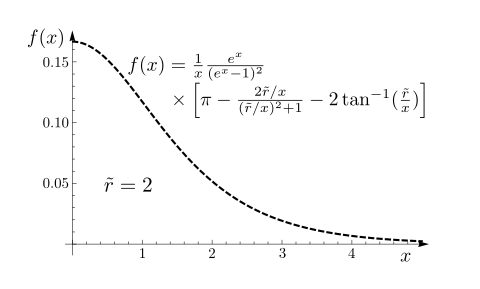
\includegraphics[width=0.49\textwidth]{behaviour_integrand.pdf}}
	\subfigure[]{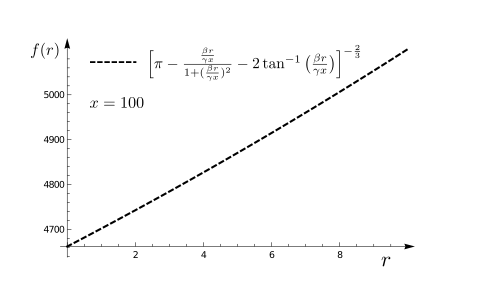
\includegraphics[width=0.49\textwidth]{dependence_integrand.pdf}}
	\caption{caption}
	\label{fig:behaviour integrand}
\end{figure}
%
A solution of the integral is evaluated determining the behaviour of the expression in squared brackets.
For large values of $x$, a linear $r$-dependence is given by the power of $-\flatfrac{2}{3}$.
This is depicted in the right hand side of figure \ref{fig:behaviour integrand}, where $x$ is set to 100.
An approximated expression is generated for the interand using the method of power counting.
The initial point of this approach is the momentum integral in euqtion \eqref{eq:starting expression}.
Numerator and differatial yield in total the power of two, while the denominator generates the power of eight.
Combining both, the integrand is a function proportional to $k^{-6}$.
The further approach is now to investigate singularities of the integrand.
The limit $r \to 0$ or $\epsilon \to 0$ is seperately generated singularities in the function.
Both are considered with the power of three, since the power of them is half in comparison to the power of $k$ in equation \eqref{eq:starting expression}.
The integrand is therefore approximated by the following expression.
%
\begin{align}
	\Im{\mathcal{G}_{\dot{\mt{P}}\dot{\mt{P}}}^{\mt{ret}}(\vb{k}, z)} &\approx 
		-\frac{2 \vert \mt{J}_{\vb{G}} \vert^{2} \cdot G_{j}^{2}}{\gamma \pi^{2}} \cdot 
		\frac{\omega}{T}
		\int\limits_{0}^{\infty} \dd{x}
		\frac{x^{2} e^{x}}{(e^{x} - 1)^{2}}
		\frac{1}{(\tilde{r}^{2} + x^{2})^{\flatfrac{3}{2}}}
\end{align}
%
In figure \ref{fig:integrand exact vs approx}, the approximated expression is confronted with the exact one.
The behaviour of both are nearly identical and the estimation is inspected as valid.
The integrand is still decreasing fast to zero for $x \to \infty$, while the upper limit is set to some arbitrary cut-off $\Lambda$.
%
\begin{figure}[t]
	\centering
	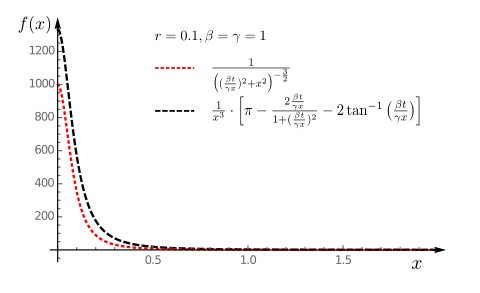
\includegraphics[width=0.6\textwidth]{original_vs_powercounting.pdf}
	\caption{caption}
	\label{fig:integrand exact vs approx}
\end{figure}
%
The ratio of the exponential functions are then expanded for small values of $x$ up to the first non-vanishing order.
The remained integral is exactly solvable and expanding the solution for small $\flatfrac{\tilde{r}}{\Lambda}$ the solution of the integral is given by
%
\begin{align}
	\Im{\mathcal{G}_{\dot{\mt{P}}\dot{\mt{P}}}^{\mt{ret}}(\vb{k}, z)} &\approx 
		-\frac{2 \gamma \vert \mt{J}_{\vb{G}} \vert^{2} \cdot G_{j}^{2}}{\pi^{2} \Lambda} \cdot \frac{\omega T}{r^{2}}
\end{align}
%
Inserting this expression and the approximated static susceptibility of \eqref{eq:static susceptibility computed} into equation \eqref{eq:static conductivity formula}, the static electrical conductivity is given by
%
\begin{align}
	\sigma_{\mt{dc}}(T) = \frac{\mu\: m_{1}\: m_{2}\: \Lambda}{2\: \gamma\: \vert \mt{J}_{\vb{G}} \vert^{2}\: G_{j}^{2}} \cdot \frac{r^{2}}{T}
\end{align}
%
Beside the temperature itself, the only temperature dependent parameter is the control parameter $r$, which is proportional to the squard inverse correlation length, $r = \xi^{-2}$.
The correlation length is originated due to the fact that the system possesses a quantum phase transition and is temperature dependent is given by $\xi = T^{-1/z}$, as shown in chapter \ref{ch:spin fermion model}.
$z$ is a critical exponent and it is chosen in dependence of the distance to the qantum critical point.
The corresponding temperature depencence of the control parameter is therefore provided to $r = T^{2/z}$.
The resistance is determined by the inverse of the conductivity.
Considering only the temperature dependent parameter, the static resistance is given by
%
\begin{align}
	\rho_{\mt{dc}}(T) \sim T^{1-\flatfrac{4}{z}}
	\label{eq:solution resistance}
\end{align}
%
Two possible choices are mentioned for the ciritcal exponent $z$ in chapter \ref{ch:spin fermion model}.
In the vicinity of the quantum critical point at higher temperatures, $z$ is chosen to be one.
The $T$-dependence of the resistance is then given by $T^{-3}$.
In the limit $T \to 0$, this is highly divergent.
$z$ is chosen to be two for lower temperatures.
Nevertheless, the $T$-dependence is evaluated to $T^{-1}$, which is still divergent in the limit $T \to 0$.

Our physial expectation is not confirmed with this divergent behaviour of the resistance.
Experiments of the investigated metals \cite{Loehneysen} are shown a linear temperature dependence of the resistance, $\rho(T) = \rho_{0} + A\: T$.
The behaviour of the resistance is described incorrect with our obtained solution \eqref{eq:solution resistance}.
A possible origin of this disgrepancy between experiemnt and theory is maybe the diagrammatic pertubation theory.
In equation \eqref{eq:Green function}, the time evolution operator is expanded up to the first non-vanishing order.
This yields the free bubble diagram, while correction to the bubble are considered  expanding the time evolutaion operator up to the next order.







%In Landau's Fermi liquid theory the resistance of a metal is given by $\rho(T) = \rho_{0} + A\: T^{2}$, where the residual resistance due to impurity scattering is represented by $\rho_{0}$.
%The $T^2$-dependence is originated by electron-electron scattering and umklapp-scattering \cite{Bader, Pal}


%In \cite{Loehneyesen} metals are investigated where a non-Fermi liquid behaviour 
%The consideration of umklapp scattering 

%Both results do not describe the physical results, presented in \cite{Loehneysen}.
%Here, 

%coincide 



















%
\cleardoublepage
%
%
\chapter{Conclusion}
\label{ch:conclusion}
%
%
Metals and alloys are described by the spin-fermion-model at the vicinity of a quantum critical point, as suggested by \cite{Abanov&Chubukov&Schmalian}.
Spin fluctuations are generated at the transition from the paramagnetic to the antiferromagnetic phase near absolute zero.
Large momentum $\vb{Q}$ is carried from these spin density waves and an interaction between fermions on the Fermi surface at $\vb{k}$ and $\vb{k}+\vb{Q}$ is therefore effected by them.
The corresponding free spin density propagator, depicted in equation \eqref{eq:undamped spin propagator}, is calculated by us and his periodicity is also shown, using the equation of motion for Green functions.

The microscopic origin of spin fluctuations is due to permanent particle-hole excitations around the Fermi surface.
An interaction between spin density waves and partile-hole excitations is also present.
As a consequence of this interplay between spin fluctuations and fermions, damping is considered for the spin density waves.
The inverse lifetime of the spin fluctuation is corresponding to the full renormalized fermion bubble since they possess no own damping source
The damping term $\gamma|\omega_{n}|$ is calculateded using diagrammatic technique, where $\gamma$ is a damping constant and $\omega_{n}$ a Matsubara frequency (see equation \eqref{eq:damped spin propagator}).
The periodicity of the spin propagator is not changed due to damping.

Additionally, conservation of momentum and current is proved in two cases: In the unperturbed spin-fermion-model and under consideration of umklapp scattering.
The Heisenberg equation of motion is used to compute the time derivatives of both quantities.
In the unpertubated system the momentum is a conserved and the current is a unconserved quantity (see equations \eqref{eq:time derivative momentum} and \eqref{eq:time derivative current}).
Considering umklapp scattering the momentum is also a unconserved quantity (see equation \eqref{eq:time derivative momentum finite}), while current and its time derivative is unmodified.

In chapter \ref{ch:infinite conductivity} and \ref{ch:calculation} the static electrical conductivity is caluculated for two cases:
1) For a system with conserved momentum and non-conserved current and
2) for a system perturbed by umklapp scattering.
The memory-matrix-formalism, introduced by Mori \cite{Mori} and presented well by Forster \cite{Forster}, is used for our computation.
Autocorrelation functions are depending on a memory function $\mt{M}(z)$ and living in the Liouville space.
The latter is a vector space that has operators acting on an usual quantum mechanical Hilbert sapce as basis vectors.
The history of the autocorrelation function is described by the memory function which decays exponentially.
This is not the case for conserved quantities and the time evolution of correlation functions is therefore described correct also in the limit $t\to\infty$ or $\omega\to0$.
In chapter \ref{ch:infinite conductivity} it is shown that the static conductivity attains a infinite value in the case of conserved momentum and unconserved current.
Our main calculation is presented in chapter \ref{ch:calculation}.
Similar to the treatment of Patel and Sachdev \cite{Patel&Sachdev}, the static electrical conductivity is computed for the spin-fermion-model.
Our model is modified by an anisotropic parabolical fermionic dispersion and umklapp scattering as pertubation.
The static conductivity $\sigma_{\mt{dc}}$ is proportional to the susceptibility $\chi_{\mt{JP}}$ and the inverse Green function $\mathcal{G}_{\dot{\mt{P}}\dot{\mt{P}}}(\vb{k},z)$.
$\chi_{\mt{JP}}$ is exactly calculated with the result of temperature independence.
For the Green function the ontained integral out of the diagrammatic technique is not exactly solvable.
Therefore the certain case $\vb{G}-\vb{Q}_{1} = \vb{Q}_{2} = 0$ is observed since this one possesses a strong singularity and governs therefore the behaviour.
In this case a temperature dependence of $T^{1-4/z}$ is found, where $z$ is a critical exponent.
The resistance is proportional to this Green function and possesses therefore the same temperature dependence.
For the usually used values of $z$ ($z=1$ and $z=2$) the tempreature dependence of the resistance is determined to $T^{-3}$ and $T^{-1}$, respectivily.
%The usual values for $z$ are $z=1$ or $z=2$ for higher or lower temperature,respectively, at the vicinity of the quantum critical point.
In both cases the temperature dependence is highly divergent and disagree with the expected linear temperature dependence of the resistance shown in the measurements \cite{Loehneysen}.

The computed temperature dependence is surely to divergent as to be correct.
In the diagrammatic technique the time evolution operatore containing the spin-fermion interaction $\mt{H}_{\Psi\Phi}$ is only expanded up to the zeroth order.
In our opinion, the divergent temperature dependence of the resistance is adjusted considering higher orders in the series expansion of the time evolution operator.
The question if a linear temperature dependence of the resistance in heavy-fermion system, like $\mt{CeCu}_{5.9}\mt{Au}_{0.1}$ and $\mt{CeCu}_{5.8}\mt{Ag}_{0.2}$, is caused by umklapp scattering is still unanswered.
The calculation considering higher order terms is still an interesting task for the future.















%
\cleardoublepage
\appendix							% appendix is starting
\cleardoublepage
%
%
\chapter{Properties of the Kubo Relaxation Function}
\label{app:properties of the Kubo relaxation function}
%
%
The Kubo relaxation function 
%
\begin{align}
	\Phi_{\mt{AB}}(t) = \frac{i}{\hbar} \lim\limits_{s \to 0} \int\limits_{t}^{\infty} \dd{\tau} \expval{\comm{\mt{A}_{\mt{I}}(\tau)}{\mt{B}_{\mt{I}}(0)}}_{0} e^{-s\tau}.
	\label{appeq:Kubo relaxation function}
\end{align}
%
is introduced in section \ref{sec:kubo relaxation function} and the three relations below are still supposed.
%
\begin{enumerate}
	\item $\begin{aligned}[t] \chi_{\mt{AB}}(t) = -\Theta(t) \dv{t} \Phi_{\mt{AB}}(t) \end{aligned}$\hfill \refstepcounter{equation}(\theequation)\label{appeq:relation 1 between Phi and chi}
	\item $\begin{aligned}[t] \Phi_{\mt{AB}}(t = 0) = \chi_{\mt{AB}}(\omega = 0) \end{aligned}$\hfill \refstepcounter{equation}(\theequation)\label{appeq:relation 2 between Phi and chi}
	\item $\begin{aligned}[t] \Phi_{\mt{AB}}(\omega) = \frac{1}{i\omega}\big[\chi_{\mt{AB}}(\omega) - \chi_{\mt{AB}}(\omega = 0)\big]. \end{aligned}$\hfill \refstepcounter{equation}(\theequation)\label{appeq:relation 3 between Phi and chi}
\end{enumerate}
%
The evidence of these three relation is proven in this appendix.
The Kubo relaxation function is derivated with respect to the time $t$.
This yields immediatly the first relation, comparing the obtained derivative with the definition of the dynamical susceptibility \eqref{eq:dynamical susceptibilty}.
%
\begin{align}
	-\Theta(t) \dv{t} \Phi_{\mt{AB}}(t) = \frac{i}{\hbar} \Theta(t) \expval{\comm{\mt{A}_{\mt{I}}(t)}{\mt{B}_{\mt{I}}(0)}}_{0} = \chi_{\mt{AB}}(t)
	\label{eq:proof relation 1}
\end{align}
%
For the evidence of the second relation, the kubo relaxation function is evaluated for the time $t=0$.
The limit $\lim_{\omega\to0} \exp(i\omega \tau)$ is inserted and the lower limit of the integral is set to minus infinity, introducing the $\theta$-distribution $\theta(\tau)$.
In the last step equation \eqref{eq:proof relation 1} and the Laplace transformation are used.
%
\begin{align}
	\Phi_{\mt{AB}}(t=0) &= \frac{i}{\hbar} \lim\limits_{s \to 0} \int\limits_{0}^{\infty} \dd{\tau} \expval{\comm{\mt{A}_{\mt{I}}(\tau)}{\mt{B}_{\mt{I}}(0)}}_{0} e^{-s\tau}
	\notag \\
	\Leftrightarrow\ \Phi_{\mt{AB}}(t=0) &= \frac{i}{\hbar} \lim\limits_{\substack{s \to 0 \\ \omega \to 0}}\ \int\limits_{-\infty}^{\infty} \dd{\tau} \Theta(\tau) \expval{\comm{\mt{A}_{\mt{I}}(\tau)}{\mt{B}_{\mt{I}}(0)}}_{0} e^{i\omega \tau} e^{-s\tau}
	\notag \\
	\Leftrightarrow\ \Phi_{\mt{AB}}(t=0) &= \lim\limits_{\omega \to 0}\ \int\limits_{-\infty}^{\infty} \dd{\tau} \chi_{\mt{AB}}(\tau) e^{i\omega \tau} = \chi_{\mt{AB}}(\omega = 0)
\end{align}
%
Furthermore, the susceptibility is assumed to be good function in the sence of convergence and the limit respective to $s$ is hence taken with no doubt.
The thrid relation follows in combination of the first and second relation
Relation one is multiplied by $\exp(i\omega t)$ and is intgrated with respect to time $t$ from $0$ to $\infty$.
The definition of the Laplace transformation and integration by parts is used on the left and right hand side, respectively.
%
\begin{align}
	\int\limits_{0}^{\infty} \dd{t} \chi_{\mt{AB}}(t)\: e^{i\omega t} &= - \int\limits_{0}^{\infty} \dd{t} e^{i\omega t} \dv{t} \Phi_{\mt{AB}}(t)
	\notag \\
	\overset{\mt{PI}}{\Leftrightarrow}\ \chi_{\mt{AB}}(\omega) &= \eval{-e^{i\omega t} \Phi_{\mt{AB}}(t)}_{0}^{\infty} + i\omega \int\limits_{0}^{\infty} \dd{t} e^{i\omega t} \Phi_{\mt{AB}}(t)
	\notag \\
	\Leftrightarrow\ \Phi_{\mt{AB}}(\omega) &= \frac{1}{i\omega} \big[\chi_{\mt{AB}}(\omega) - \chi_{\mt{AB}}(\omega=0)\big]
\end{align}
%

\chapter{Analysis of Matsubara-sums}
\label{app: analysis of Matsubara-sums}

In the following appendix it is shown how to calculate two kinds of Matsubara-sums, where the diffrence is depending on the kind of singularity of thee Green-functions.
The first one have simple poles so that the sum can transform without any problems into a contour integral.
These Matsubara-sums are easy to calculate by using the residue theorem.
The second kind of sum contains one or more Green-functions, which have non-continuity at a arbitary value.
Therefore a little bit more work is to do, nevertheless the calculation isn't very complicated.
These type of singularities are called branch cuts.

\section{Simple poles} 
\label{app: simples poles}
Let us assume a Matsubara-sum like
%
\begin{align}
	S(i\omega_{n}) := \frac{1}{\beta} \sum\limits_{\omega_{n}} G(k,i\omega_{n}) e^{i\omega_{n}\tau},
\end{align}
%
where $G(k,i\omega_{n})$ is a product of Green-functions, which are analytical except single poles in the complex plane.
Often these kinds of sums appear by using Green-functions of free propagators.
The exponential function is only needed for conergent.
\endgroup
%
\cleardoublepage
\listoftodos
%
\cleardoublepage
\printbibliography
%
\backmatter
\end{document}